\sect{Ćwiczenia 1}

\begin{frame}{Zadanie 1}
	\begin{figure}
		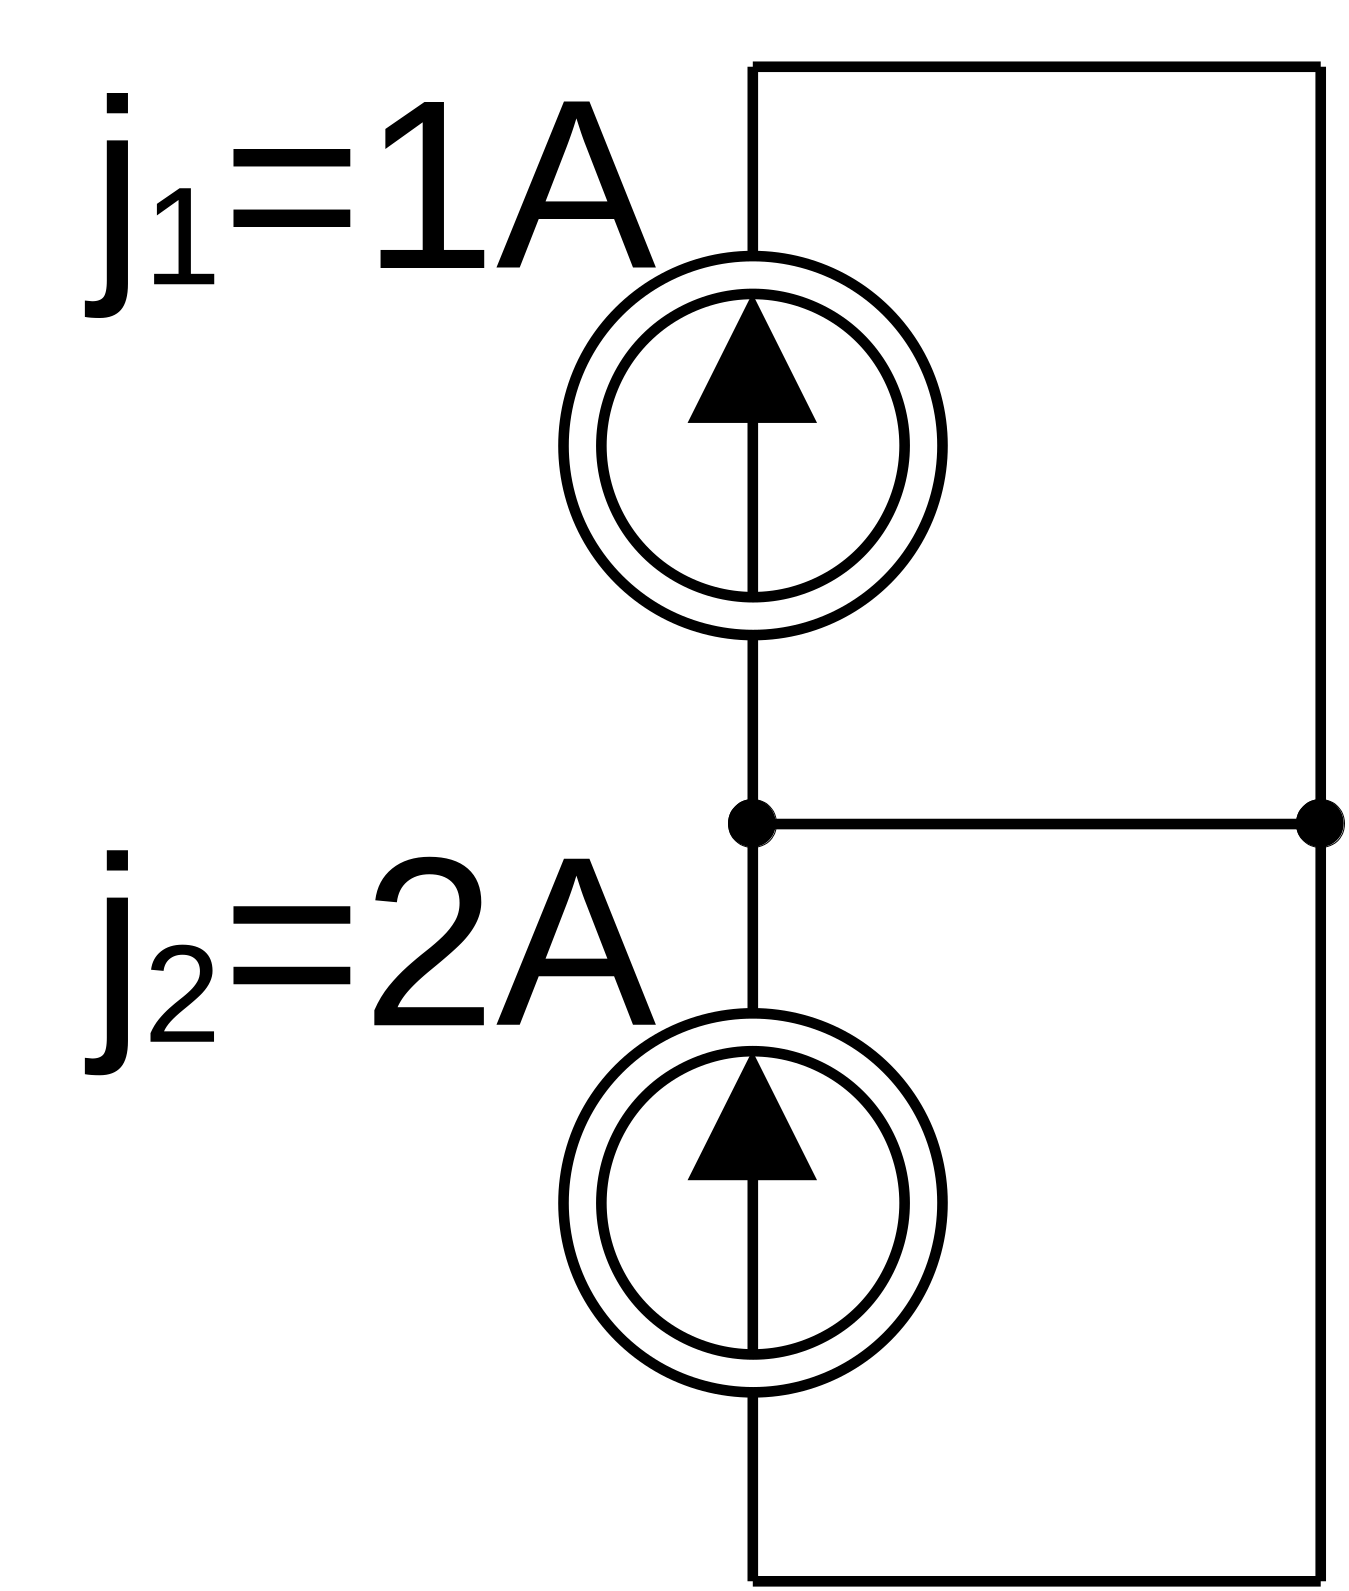
\includegraphics[scale=0.12, alt={}]{./imags/E01/01.png}
		\caption{Zadanie 1. Oblicz wszystkie prądy.}
	\end{figure}	
\end{frame}

\begin{frame}{Zadanie 2}
	\begin{figure}
		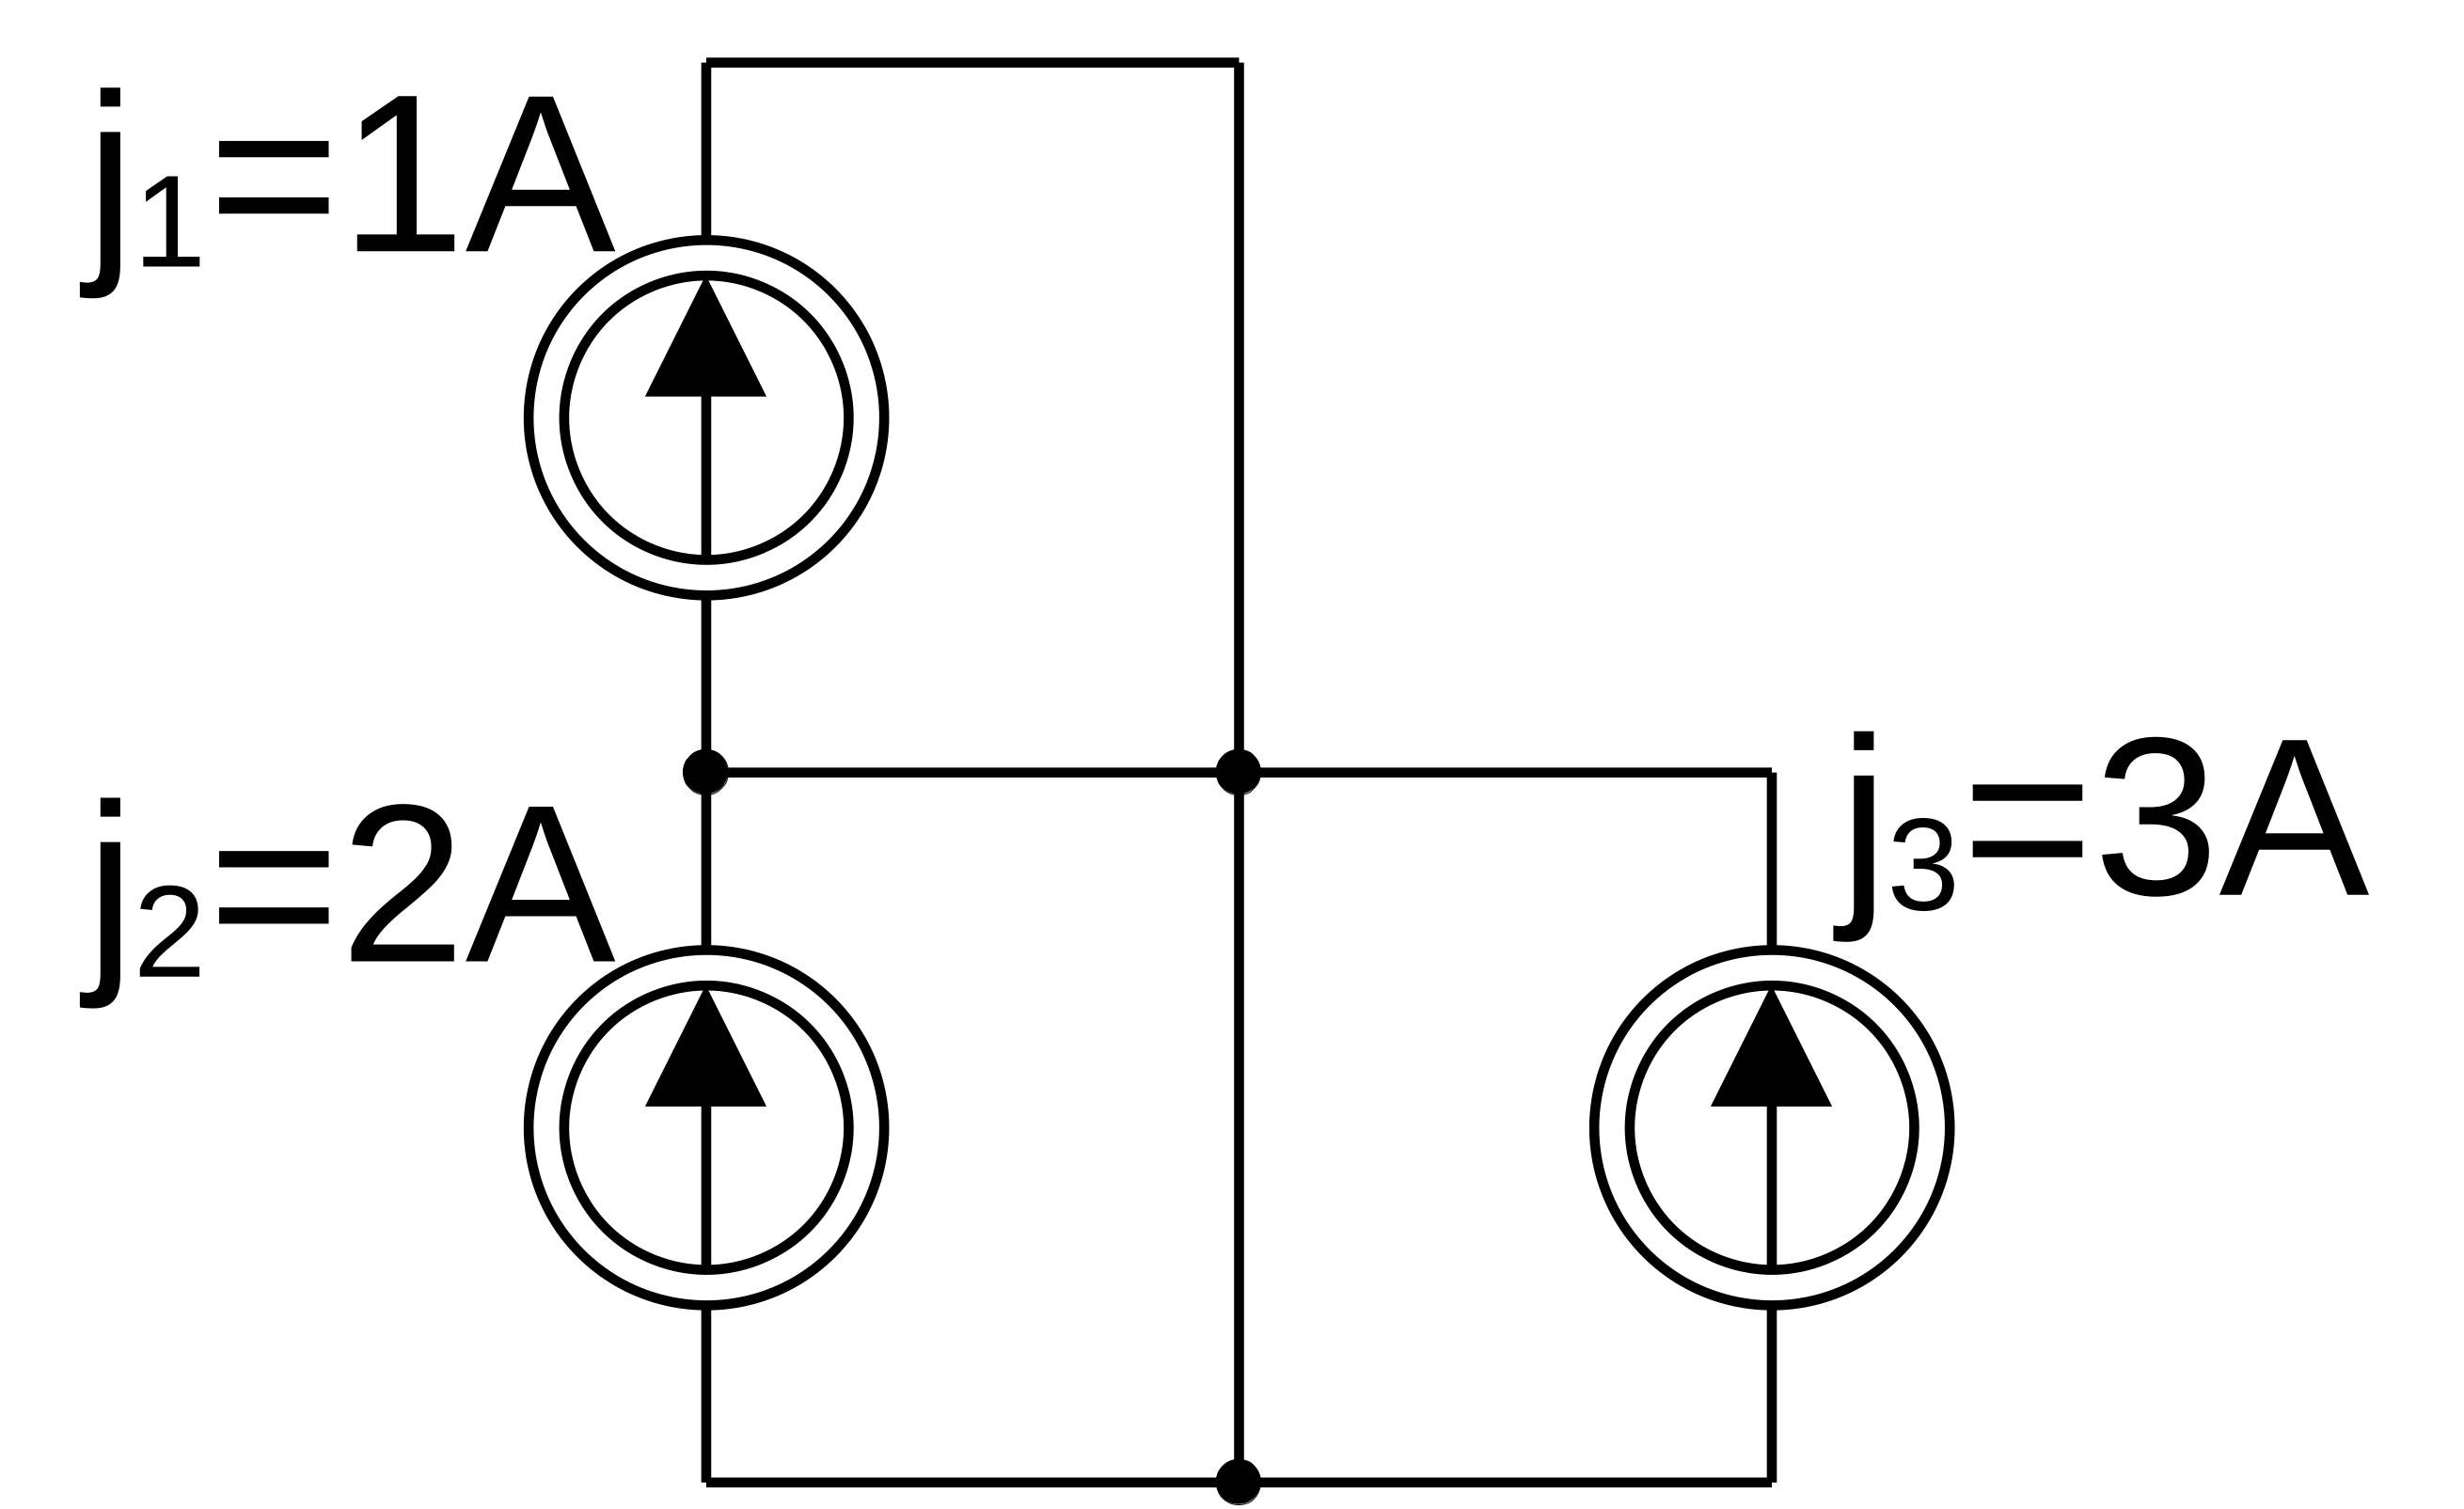
\includegraphics[scale=0.12, alt={}]{./imags/E01/02.png}
		\caption{Zadanie 2. Oblicz wszystkie prądy.}
	\end{figure}	
\end{frame}

\begin{frame}{Zadanie 3}
	\begin{figure}
		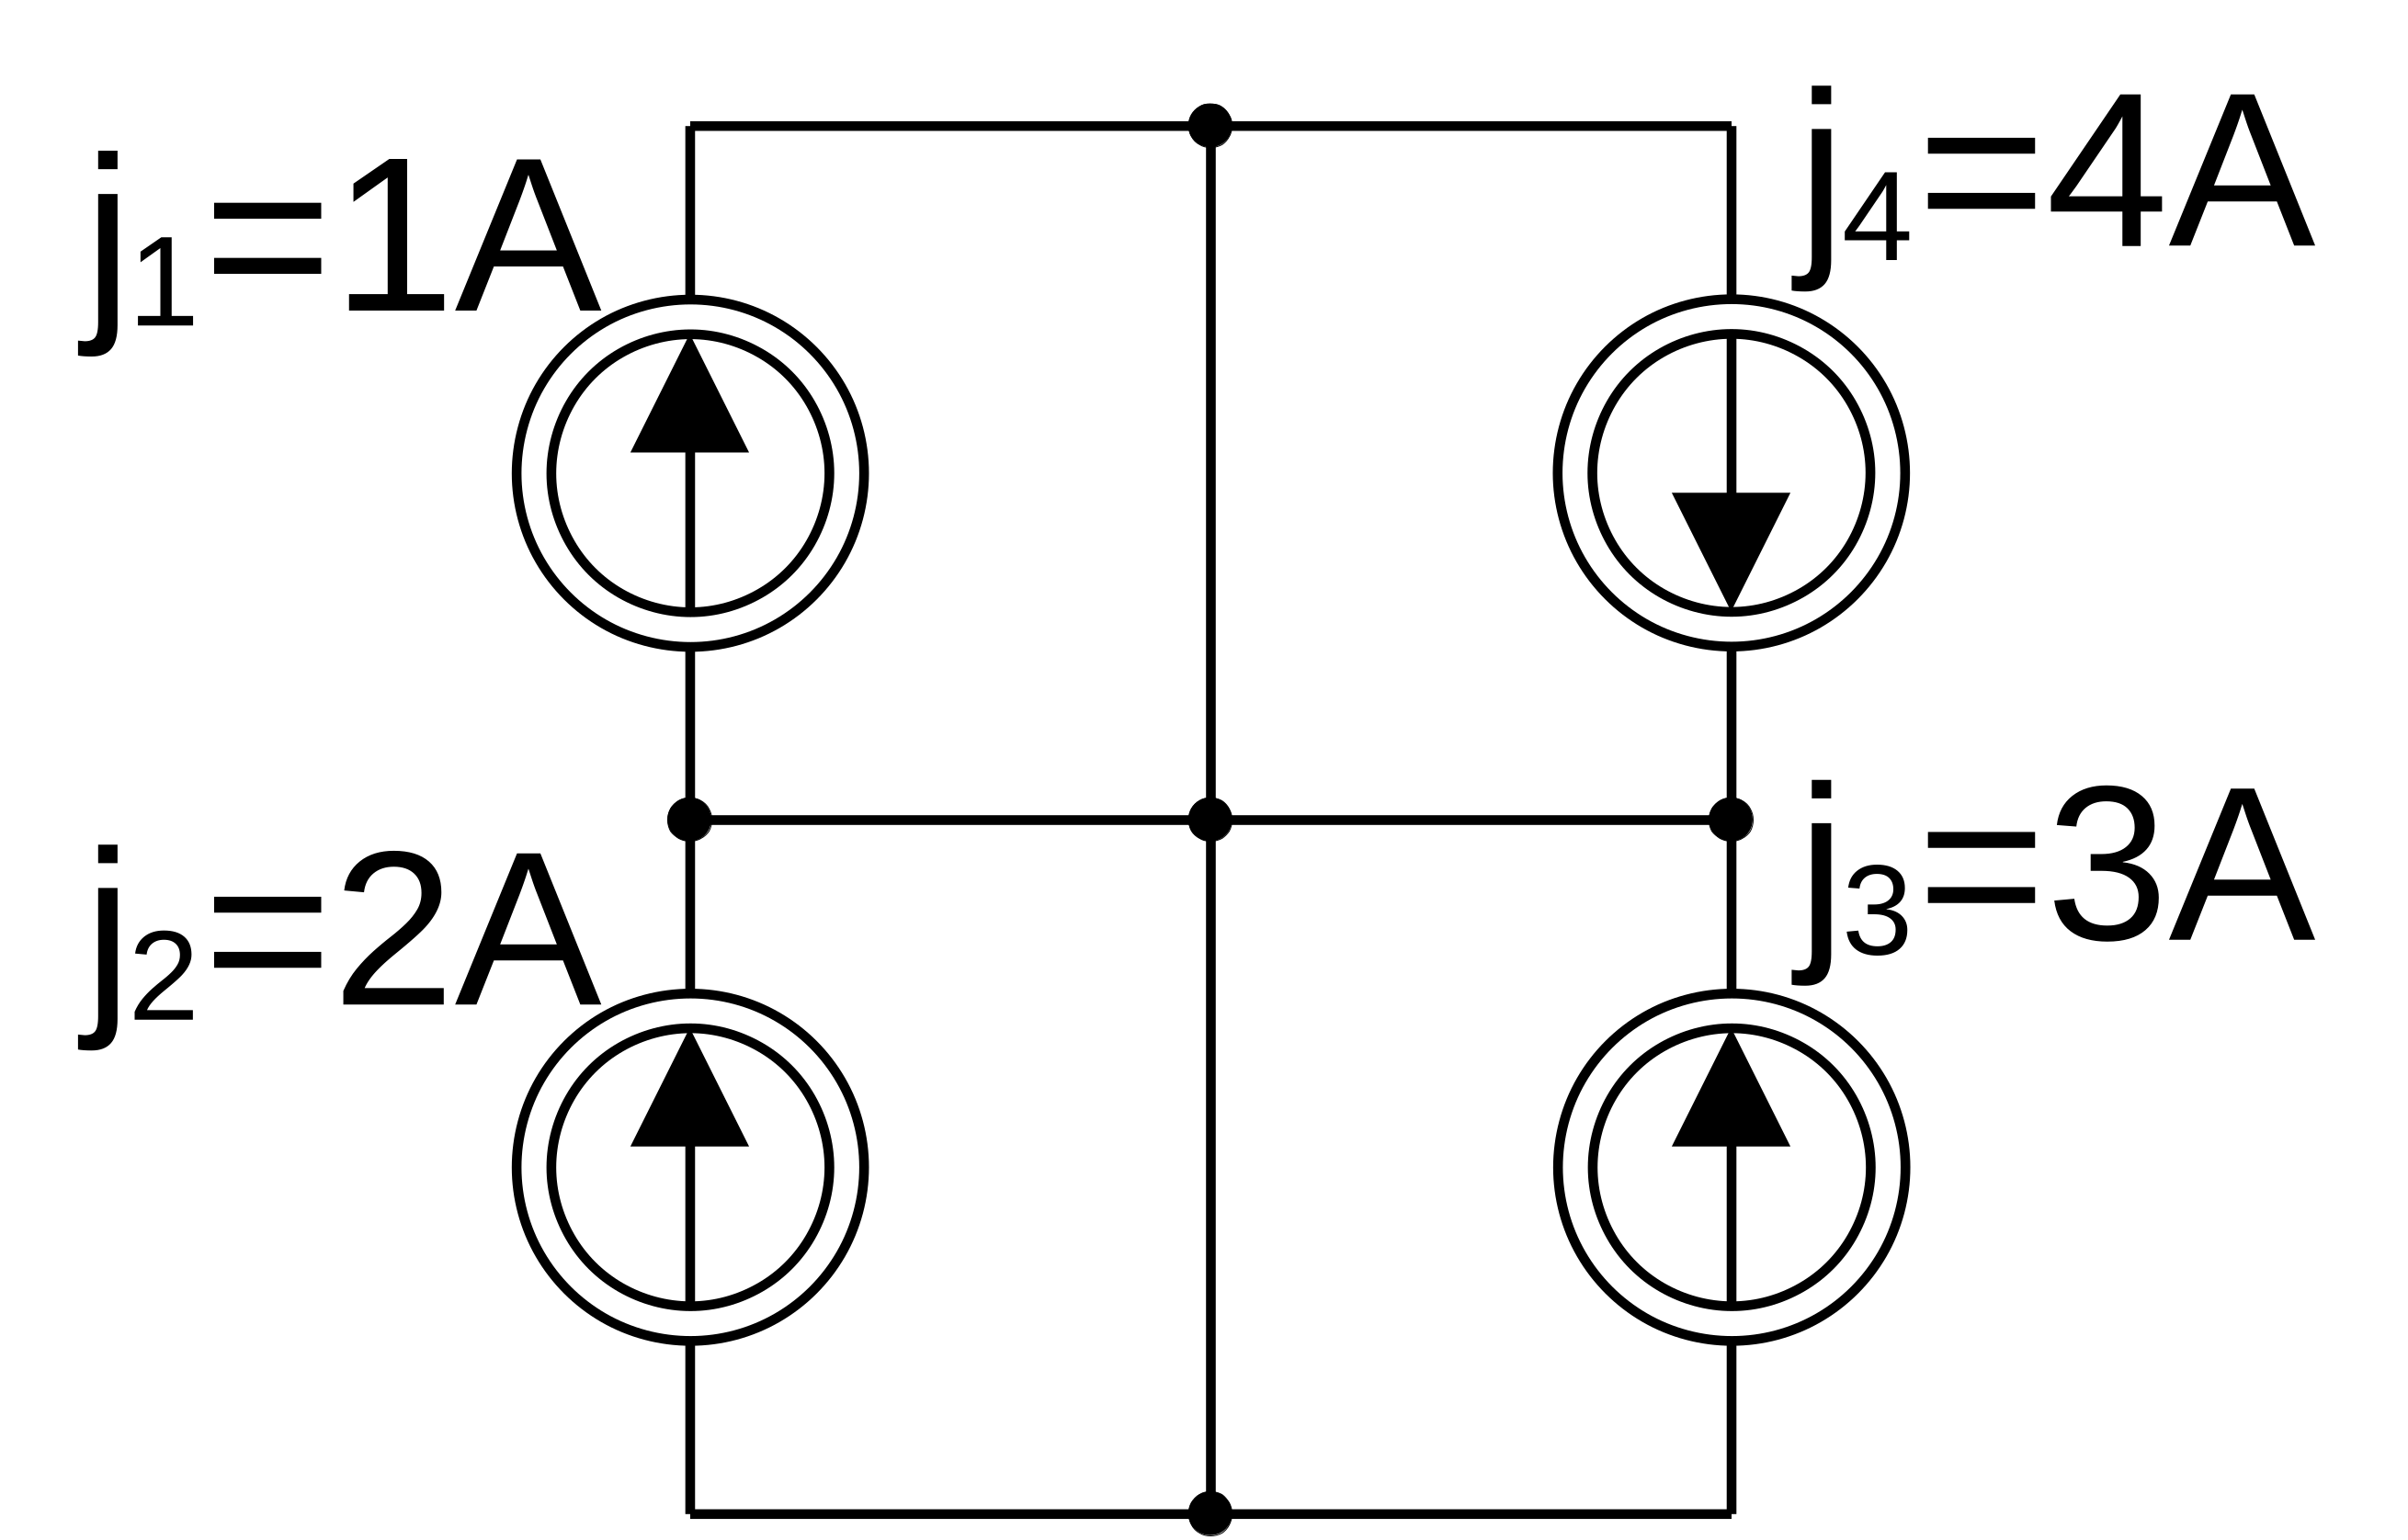
\includegraphics[scale=0.12, alt={}]{./imags/E01/03.png}
		\caption{Zadanie 3. Oblicz wszystkie prądy.}
	\end{figure}	
\end{frame}

\begin{frame}{Zadanie 4}
	\begin{figure}
		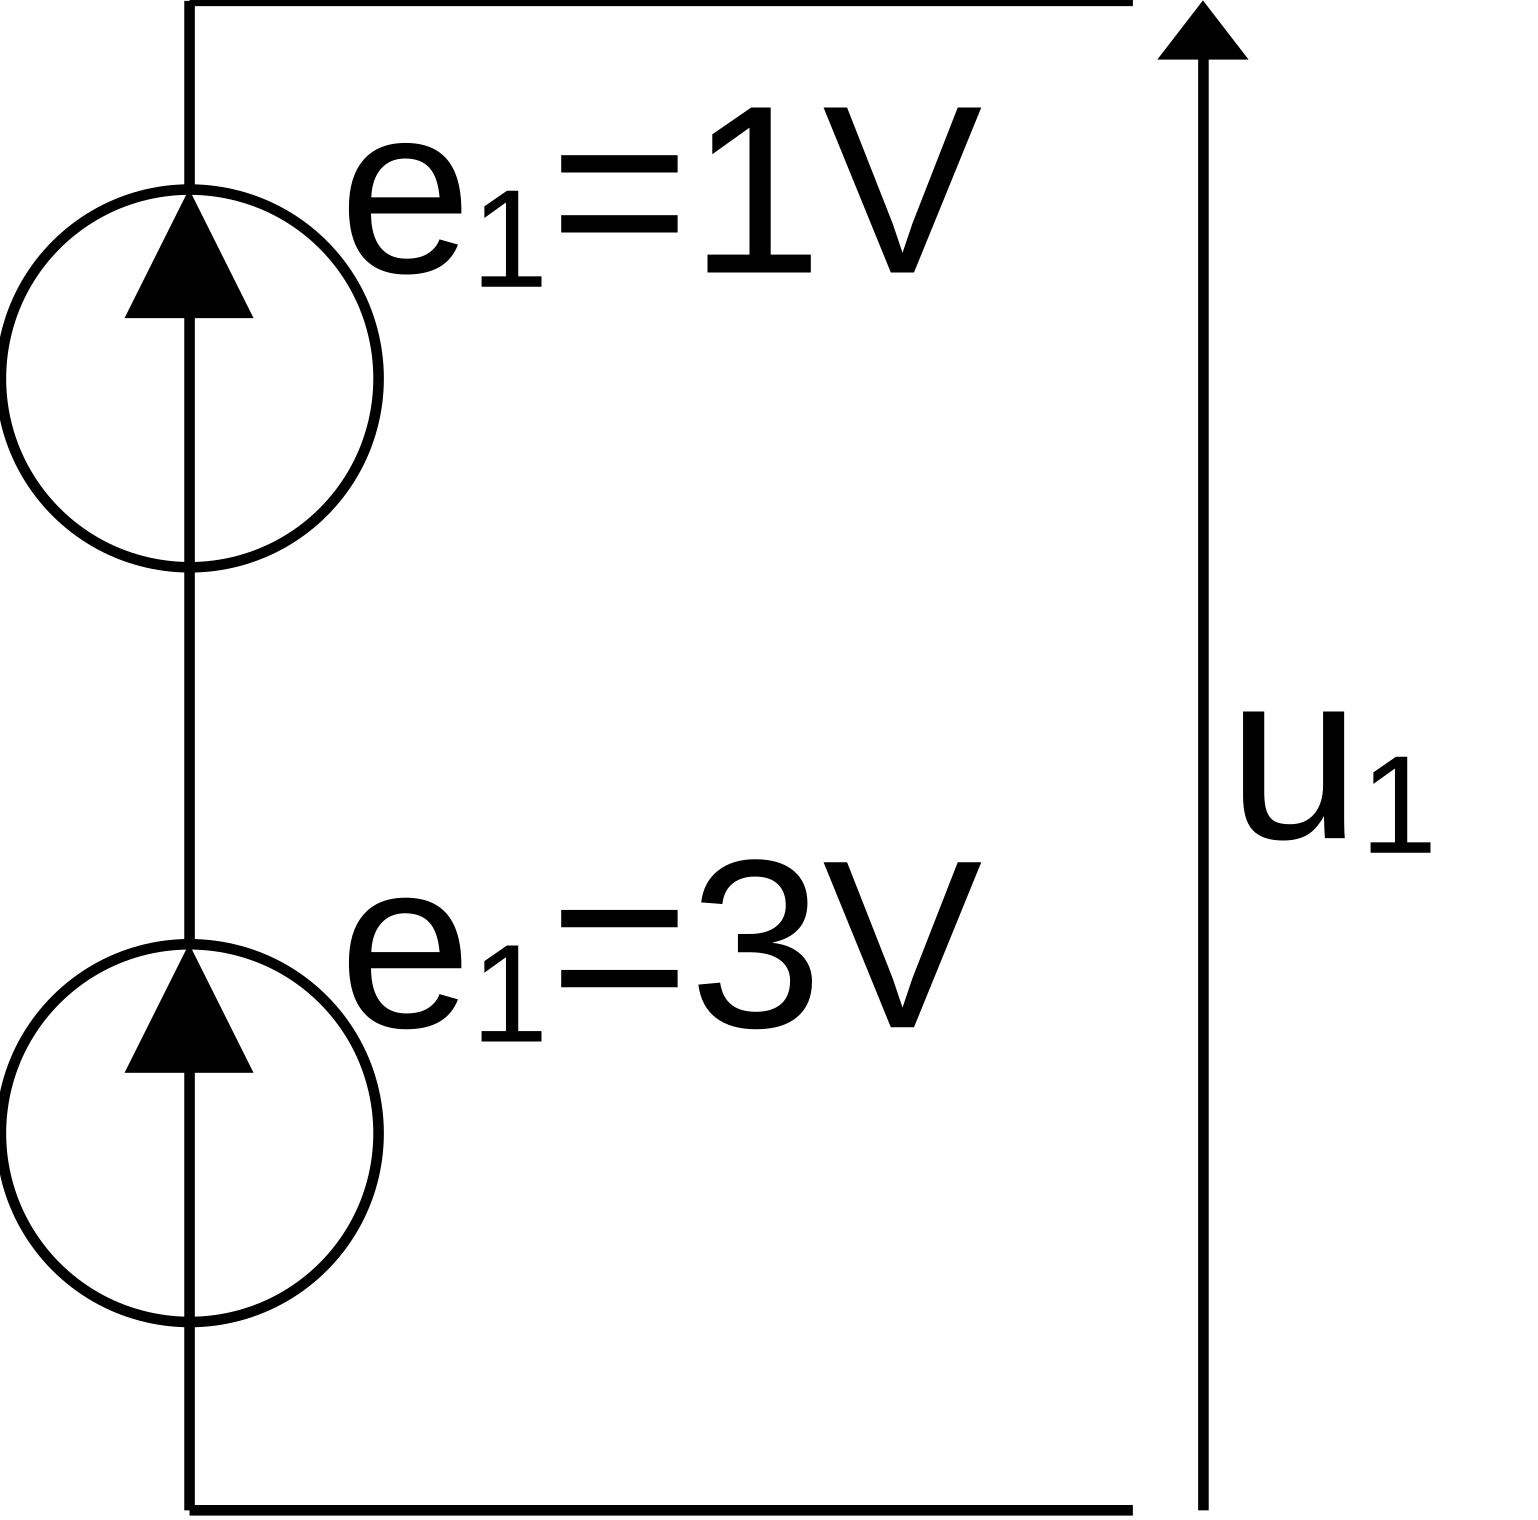
\includegraphics[scale=0.12, alt={}]{./imags/E01/04.png}
		\caption{Zadanie 4. Oblicz napięcie $u_1$.}
	\end{figure}	
\end{frame}

\begin{frame}{Zadanie 5}
	\begin{figure}
		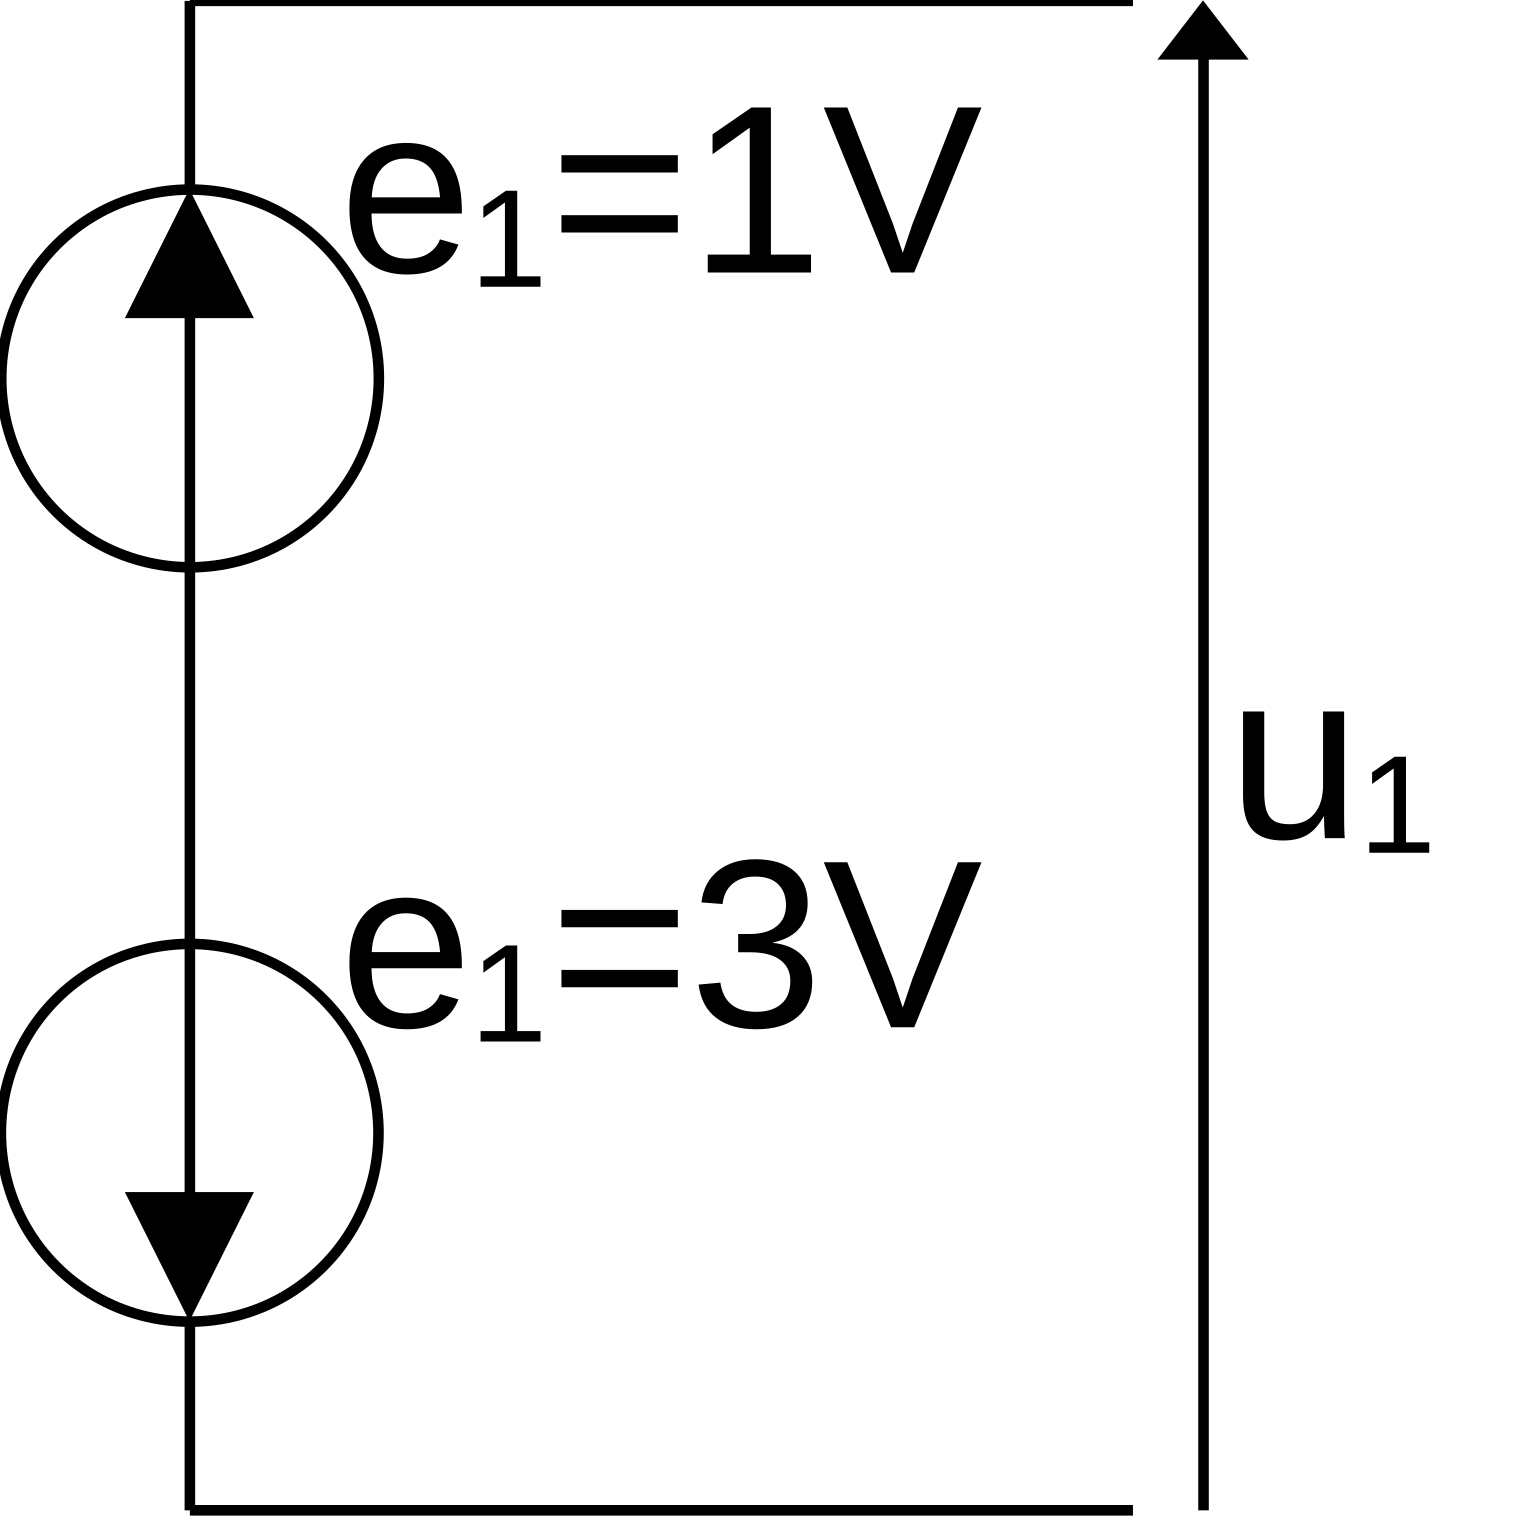
\includegraphics[scale=0.12, alt={}]{./imags/E01/05.png}
		\caption{Zadanie 5. Oblicz napięcie $u_1$.}
	\end{figure}	
\end{frame}

\begin{frame}{Zadanie 6}
	\begin{figure}
		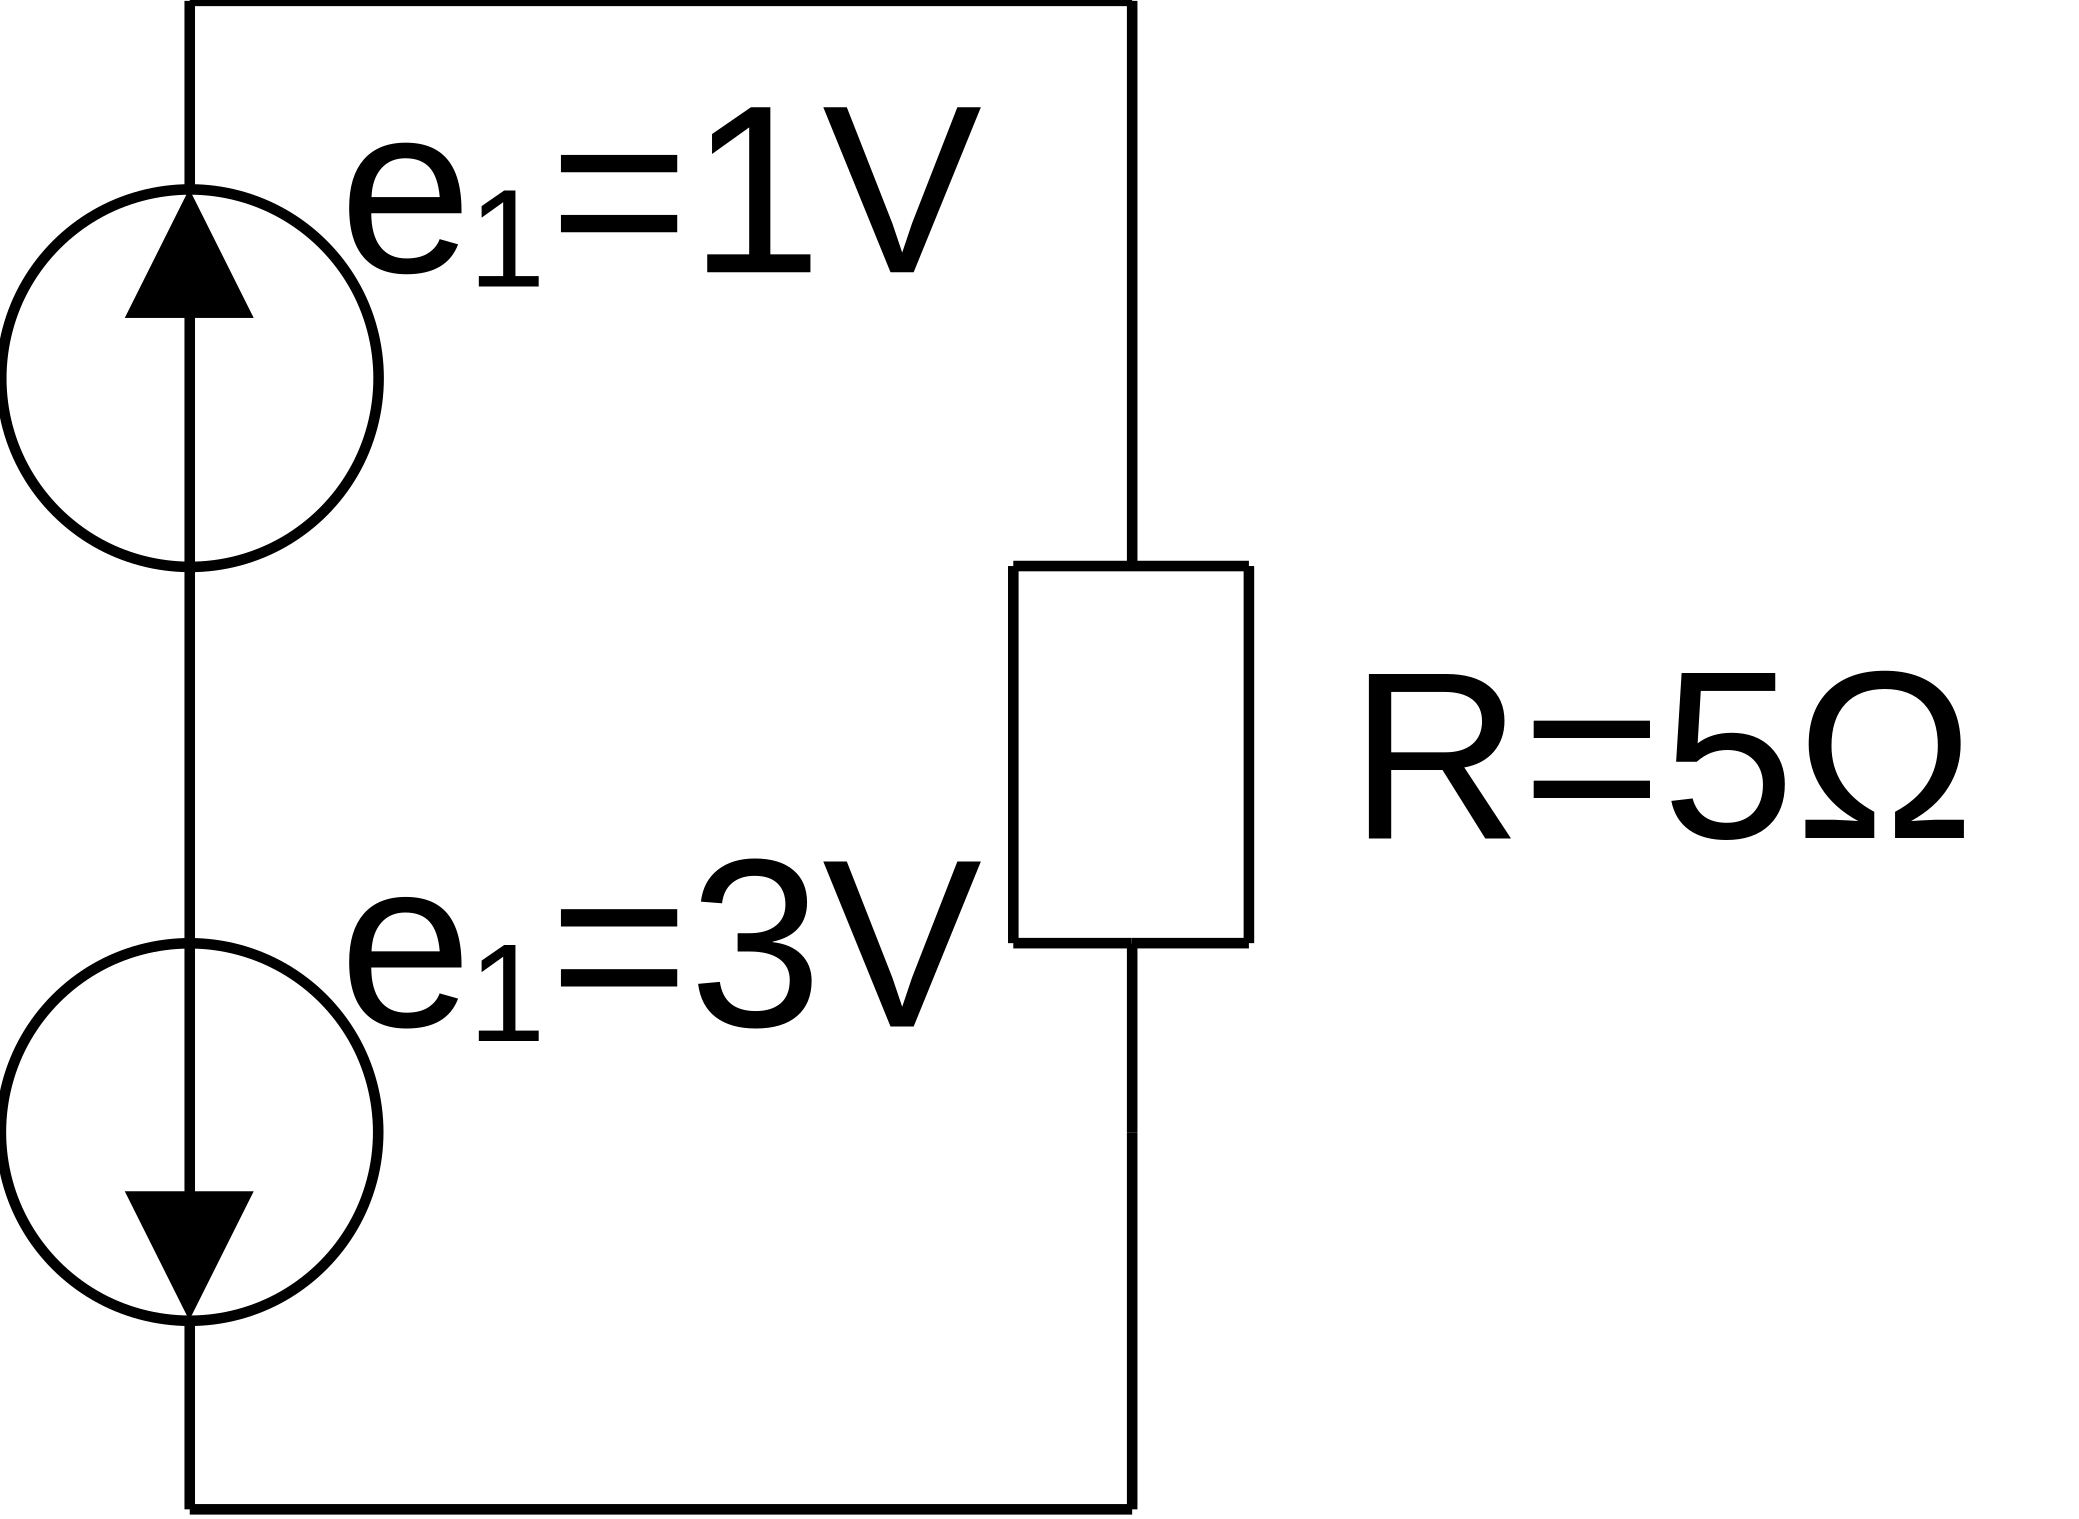
\includegraphics[scale=0.12, alt={}]{./imags/E01/06.png}
		\caption{Zadanie 6. Oblicz napięcie i prąd rezystora, wykonaj bilans mocy.}
	\end{figure}	
\end{frame}

\begin{frame}{Zadanie 7}
	\begin{figure}
		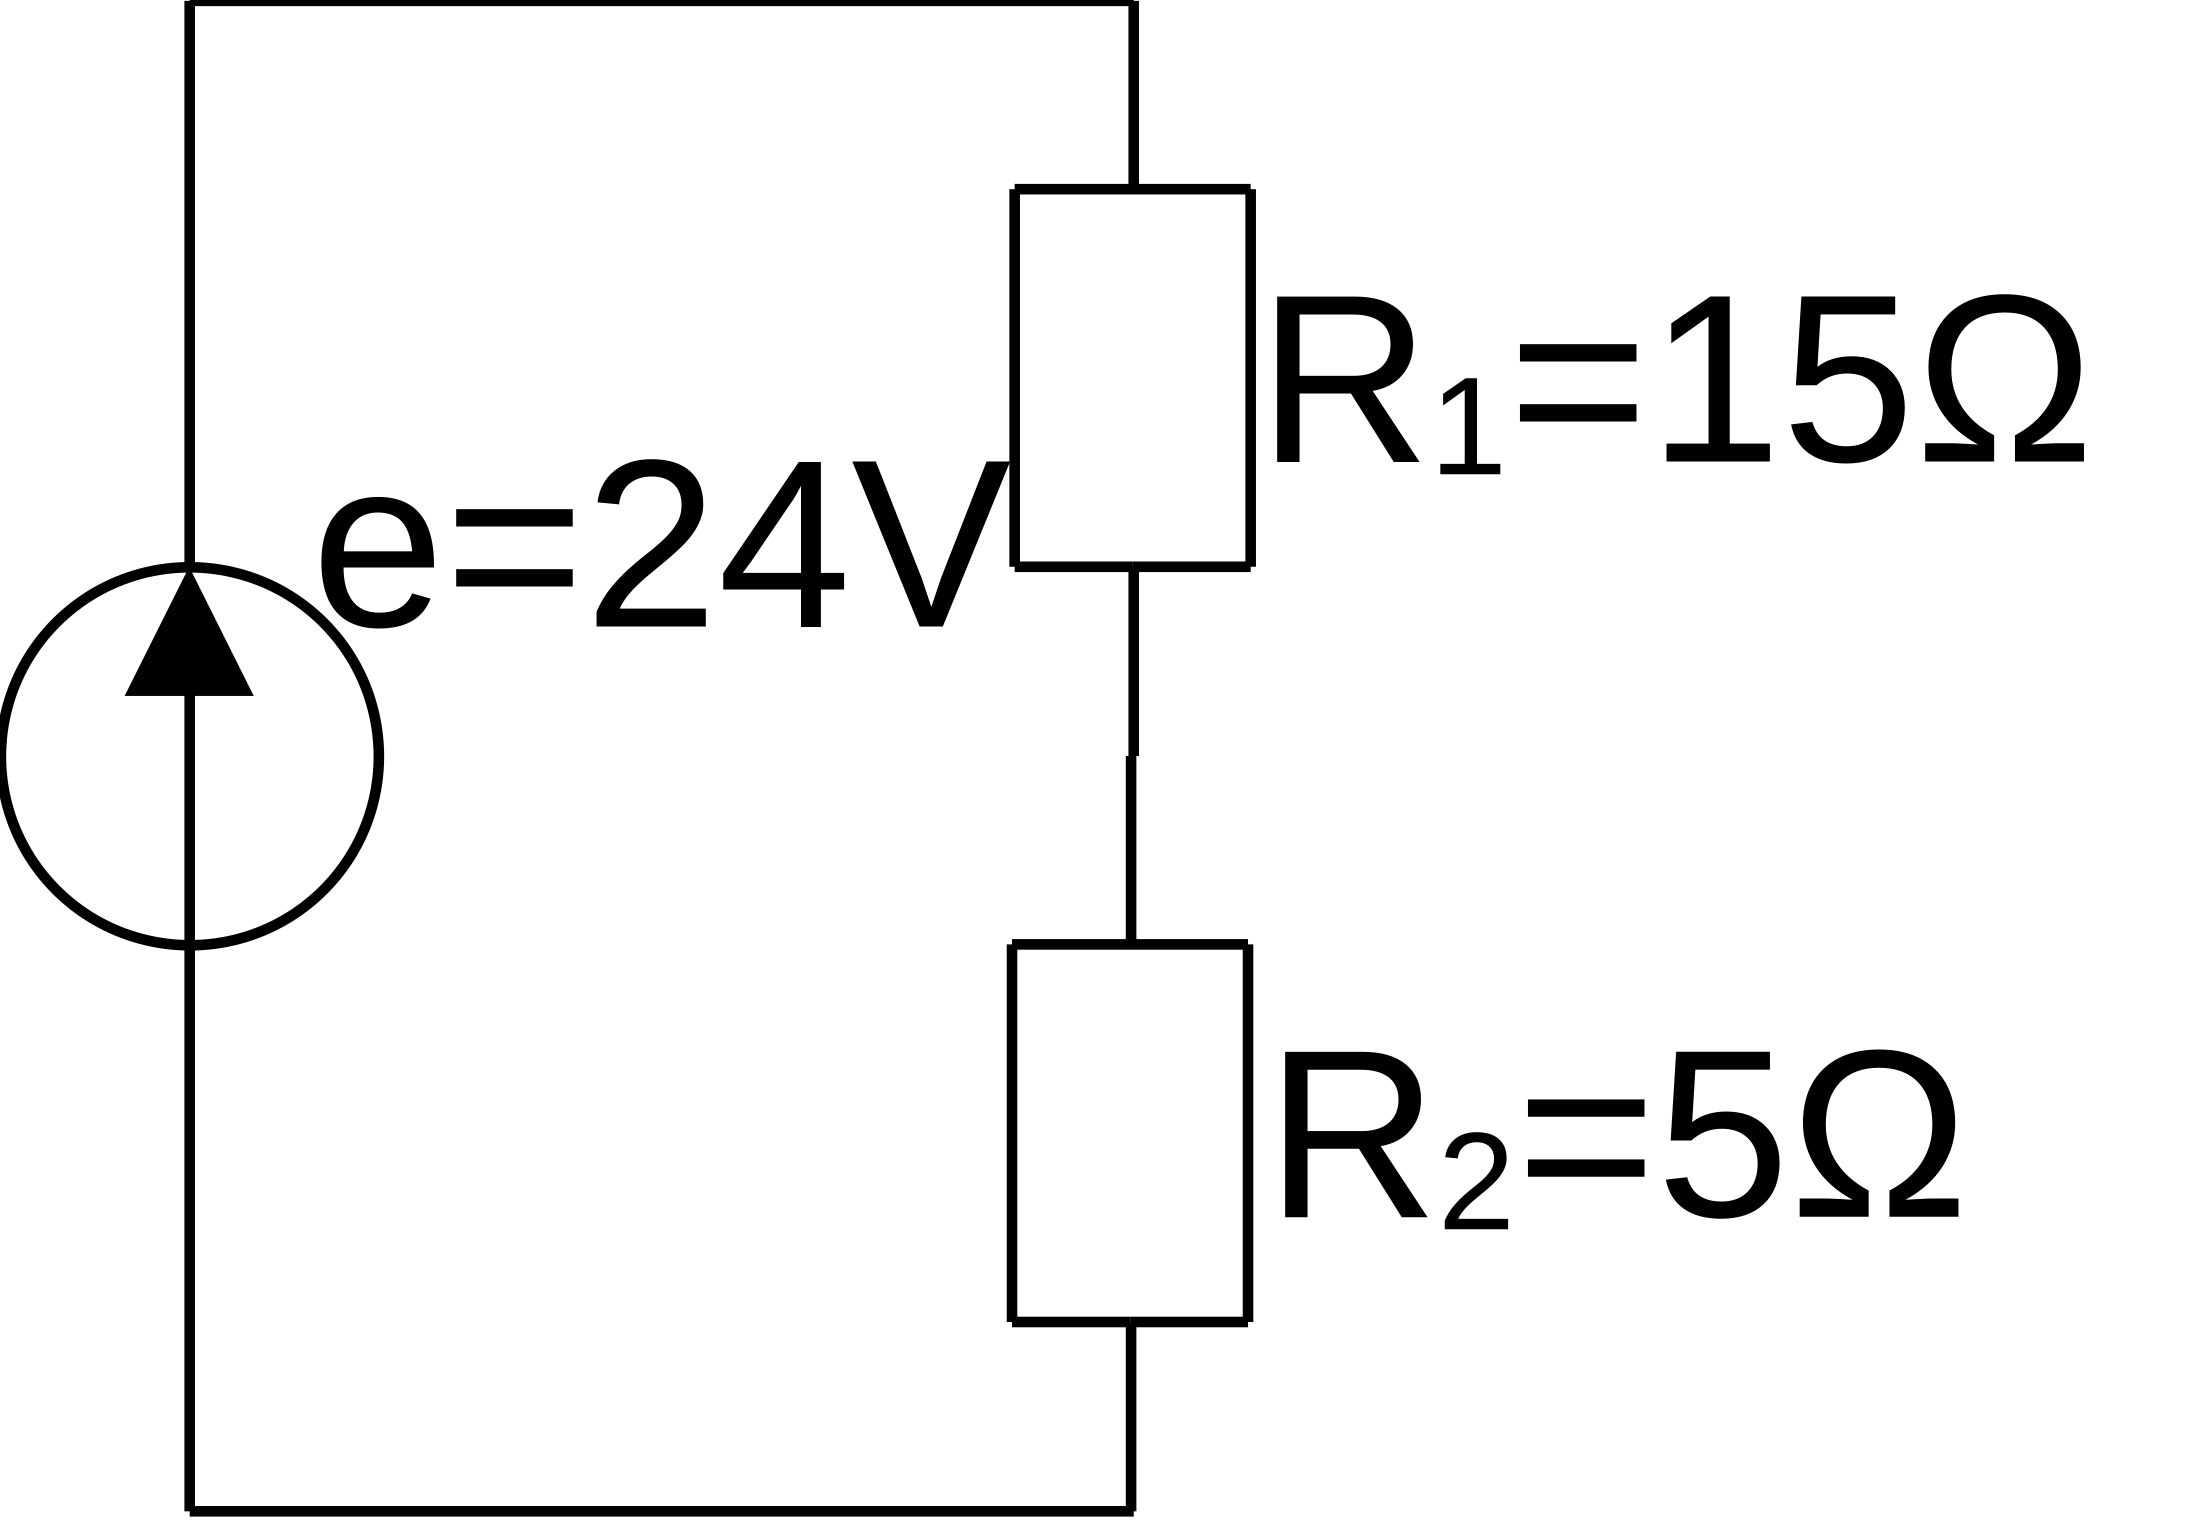
\includegraphics[scale=0.12, alt={}]{./imags/E01/07.png}
		\caption{Zadanie 7. Oblicz napięcia i natężenia rezystorów, wykonaj bilans mocy.}
	\end{figure}	
\end{frame}

\begin{frame}{Zadanie 8}
	\begin{figure}
		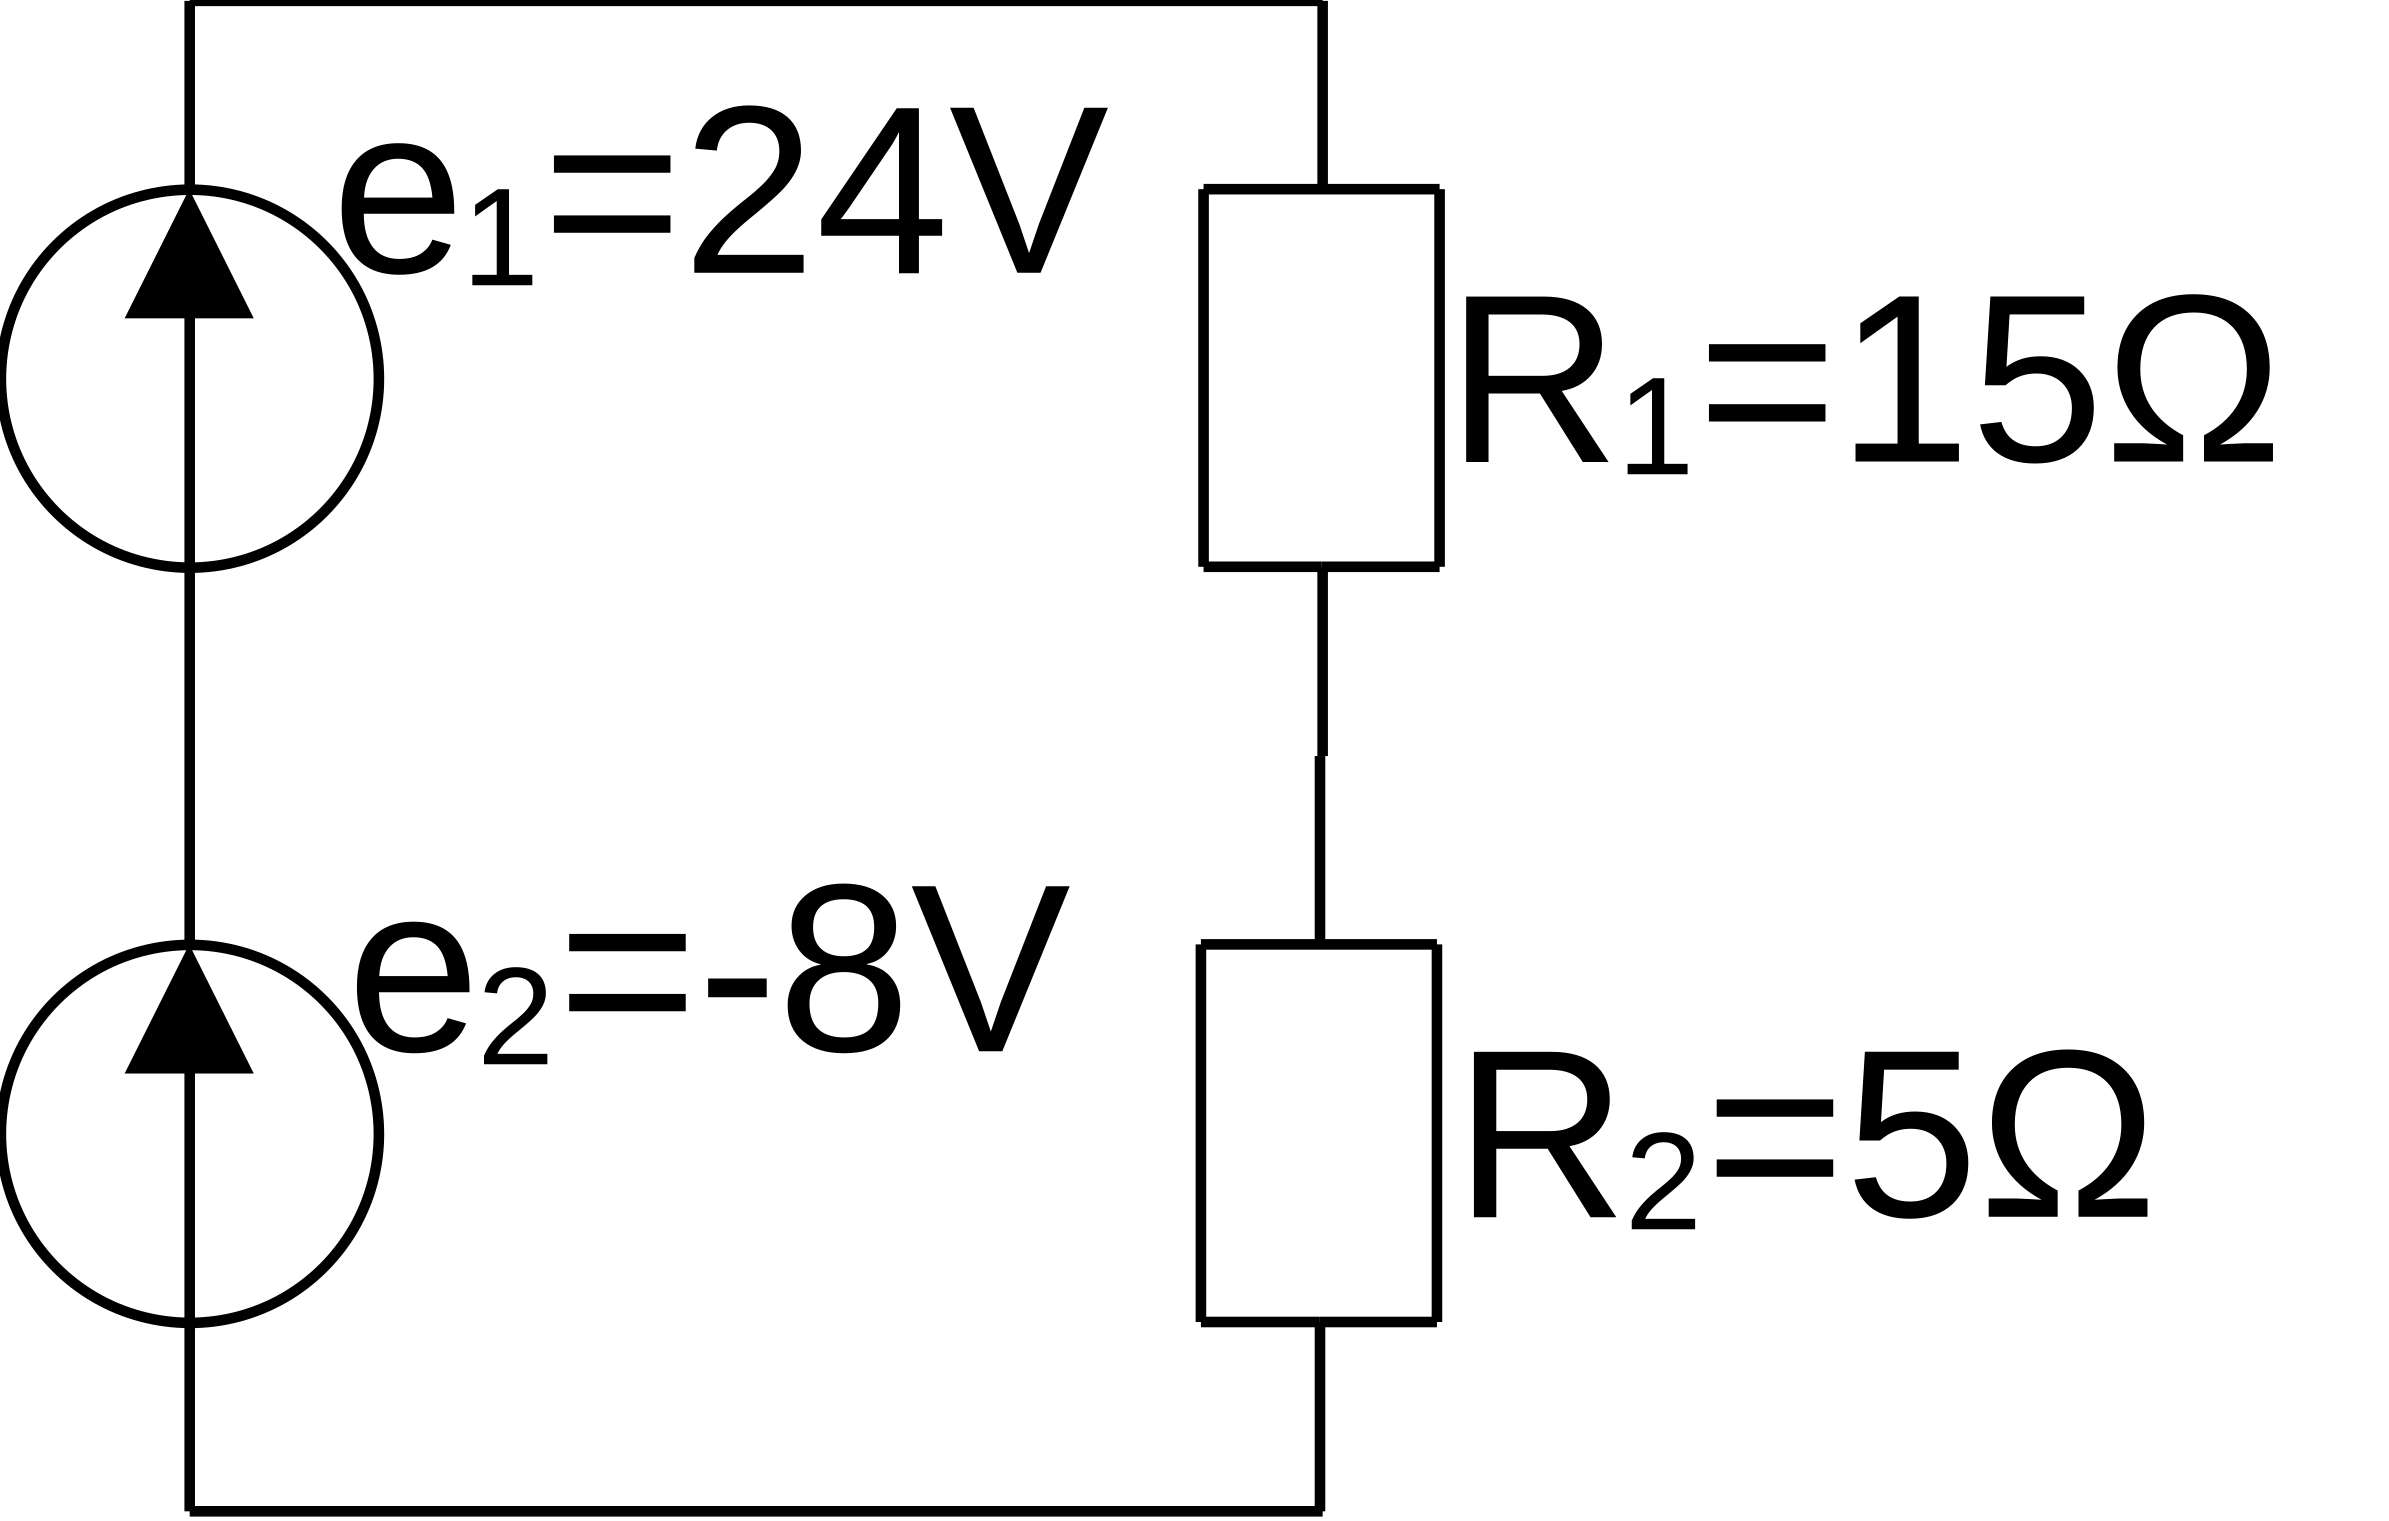
\includegraphics[scale=0.12, alt={}]{./imags/E01/08.png}
		\caption{Zadanie 8. Oblicz napięcia i natężenia rezystorów, wykonaj bilans mocy.}
	\end{figure}	
\end{frame}

\begin{frame}{Zadanie 9}
	\begin{figure}
		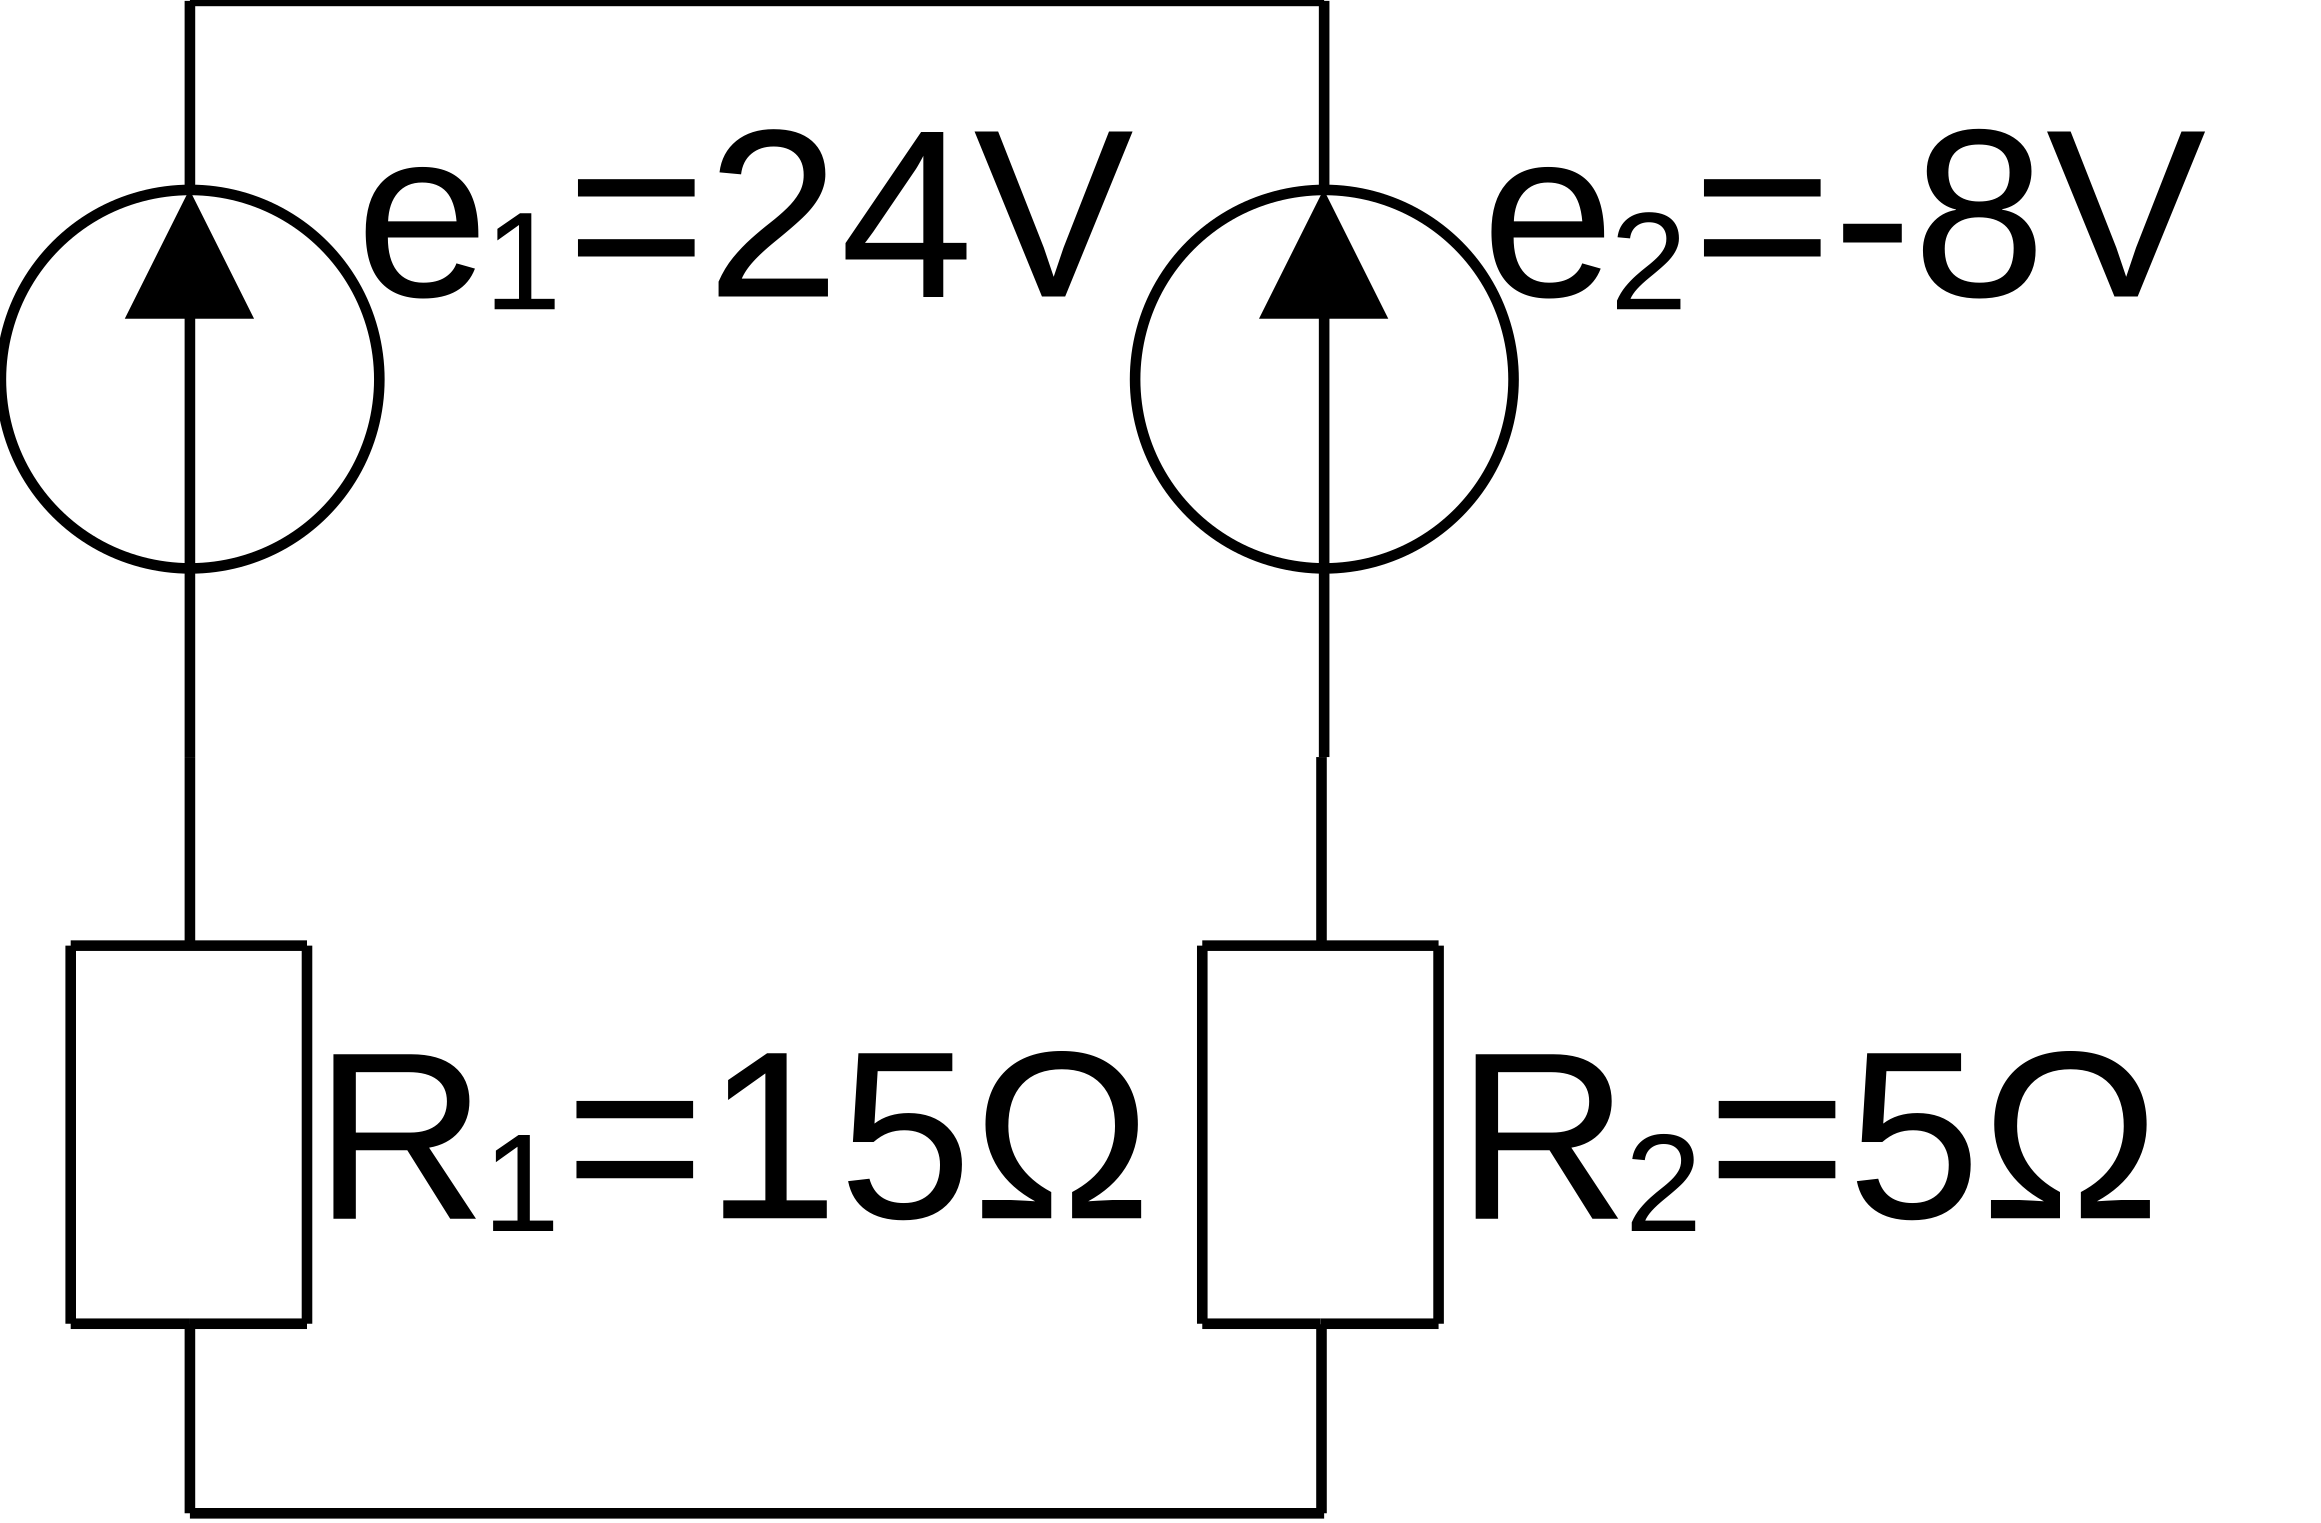
\includegraphics[scale=0.12, alt={}]{./imags/E01/09.png}
		\caption{Zadanie 9. Oblicz napięcia i natężenia rezystorów, wykonaj bilans mocy.}
	\end{figure}	
\end{frame}

\begin{frame}{Zadanie 10}
	\begin{figure}
		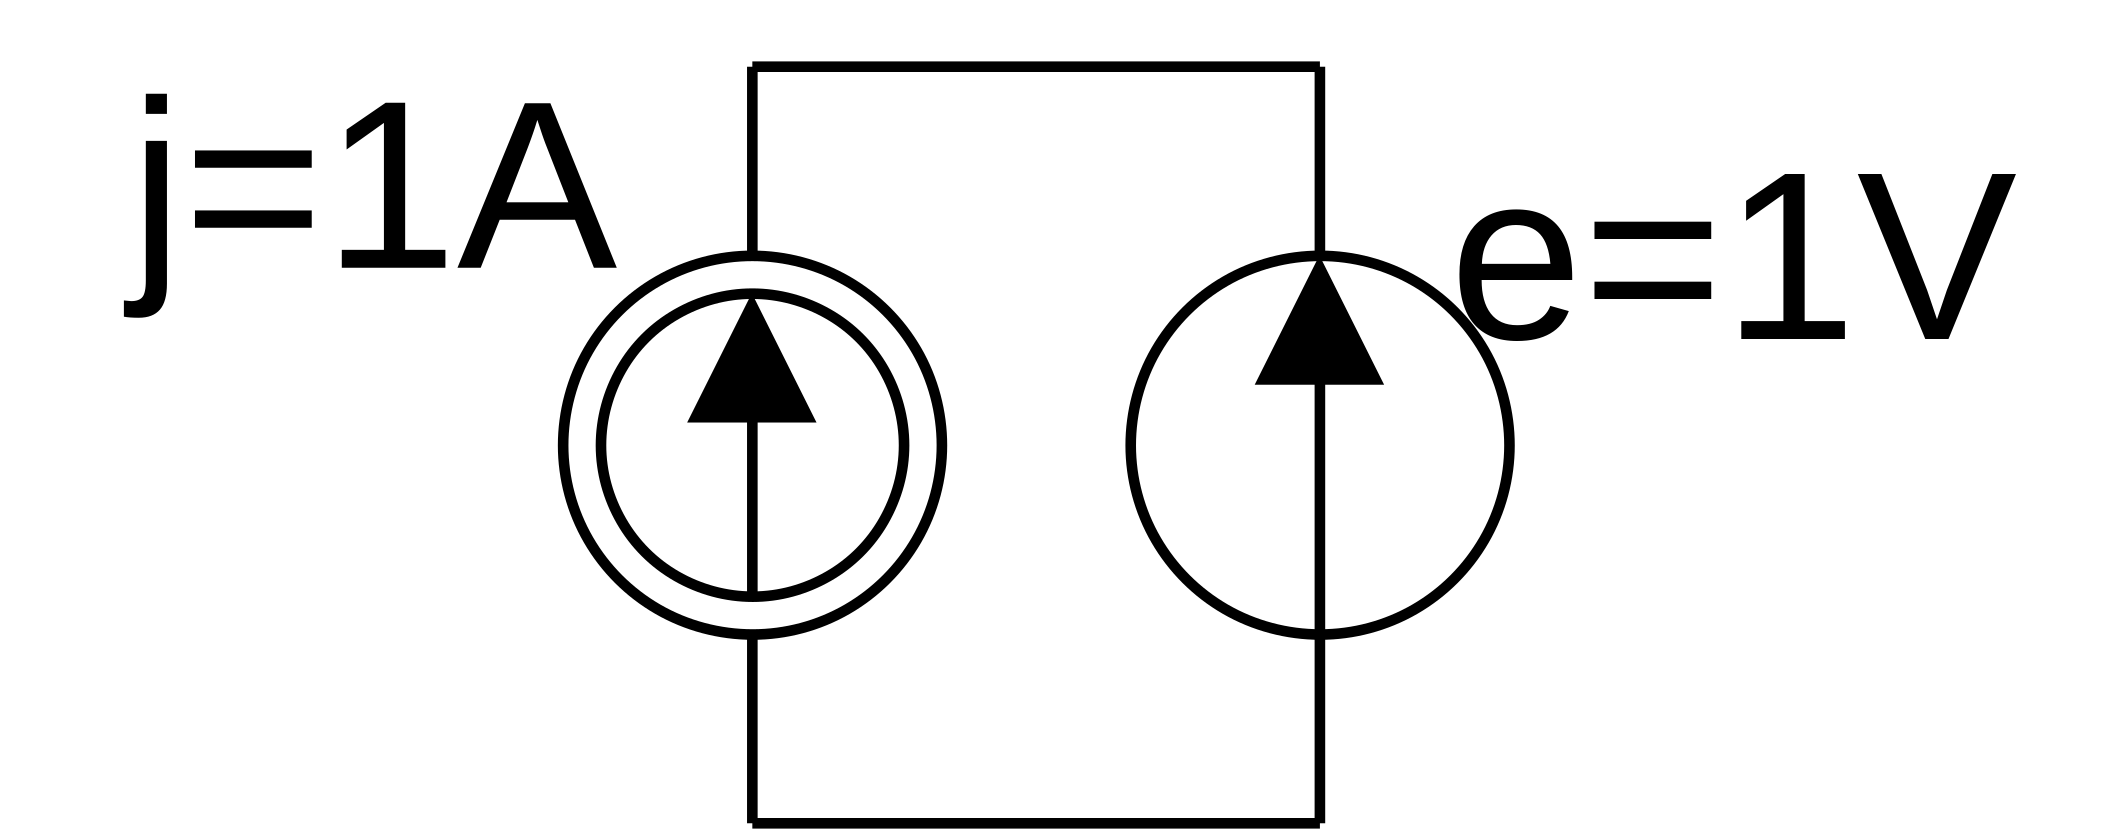
\includegraphics[scale=0.12, alt={}]{./imags/E01/10.png}
		\caption{Zadanie 10. Wykonaj bilans mocy.}
	\end{figure}	
\end{frame}

\begin{frame}{Zadanie 11}
	\begin{figure}
		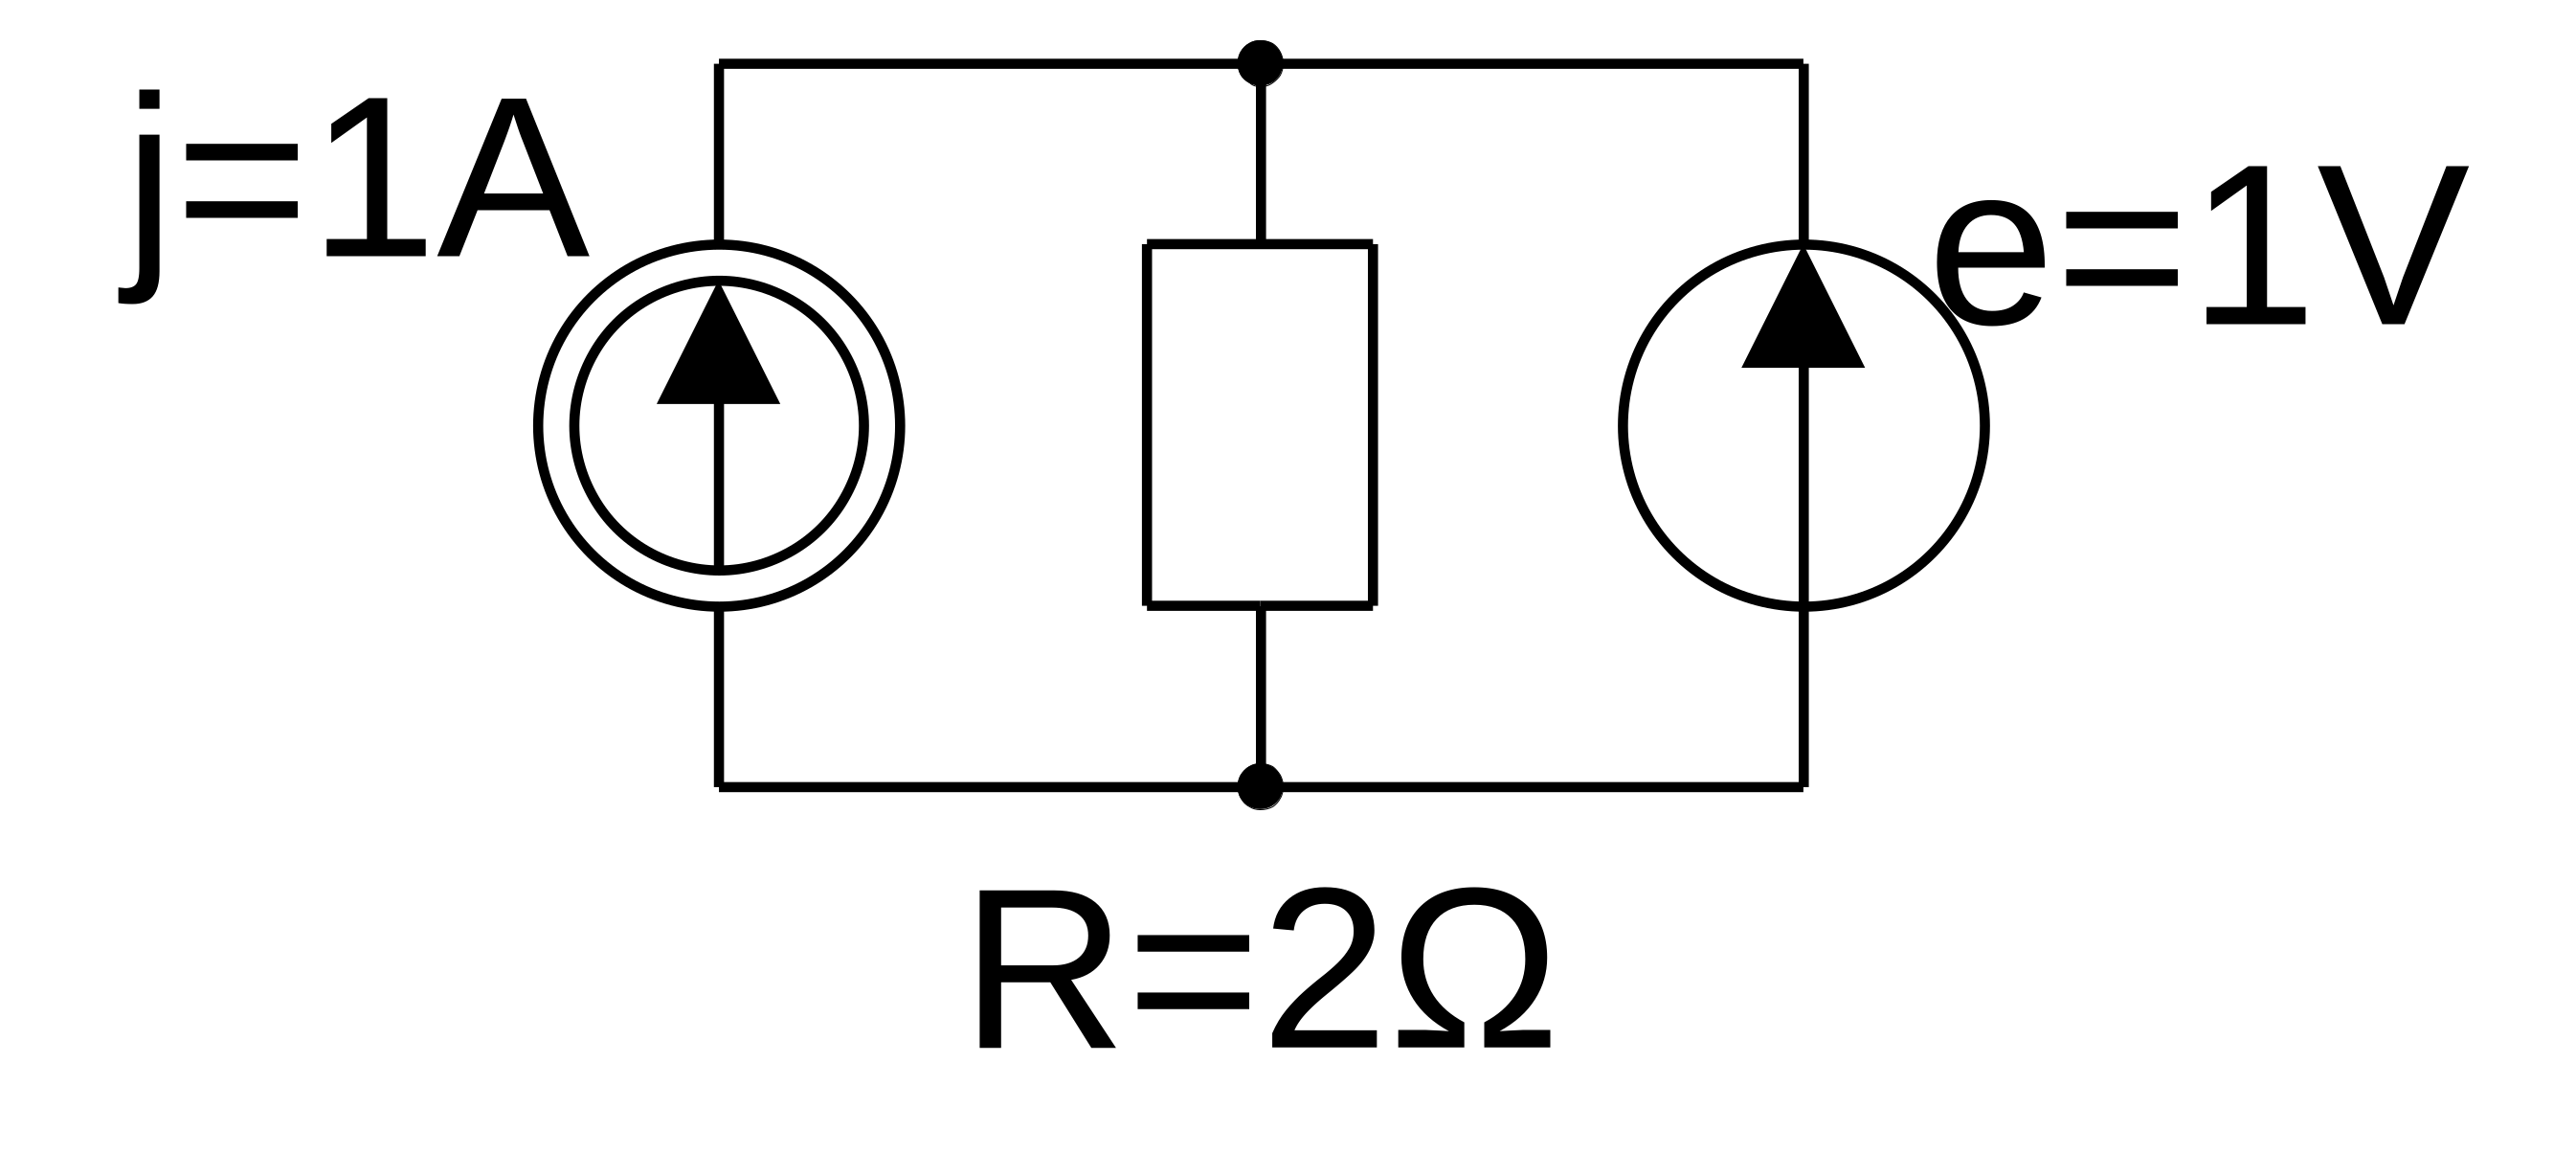
\includegraphics[scale=0.12, alt={}]{./imags/E01/11.png}
		\caption{Zadanie 11. Wykonaj bilans mocy.}
	\end{figure}	
\end{frame}

\begin{frame}{Zadanie 12}
	\begin{figure}
		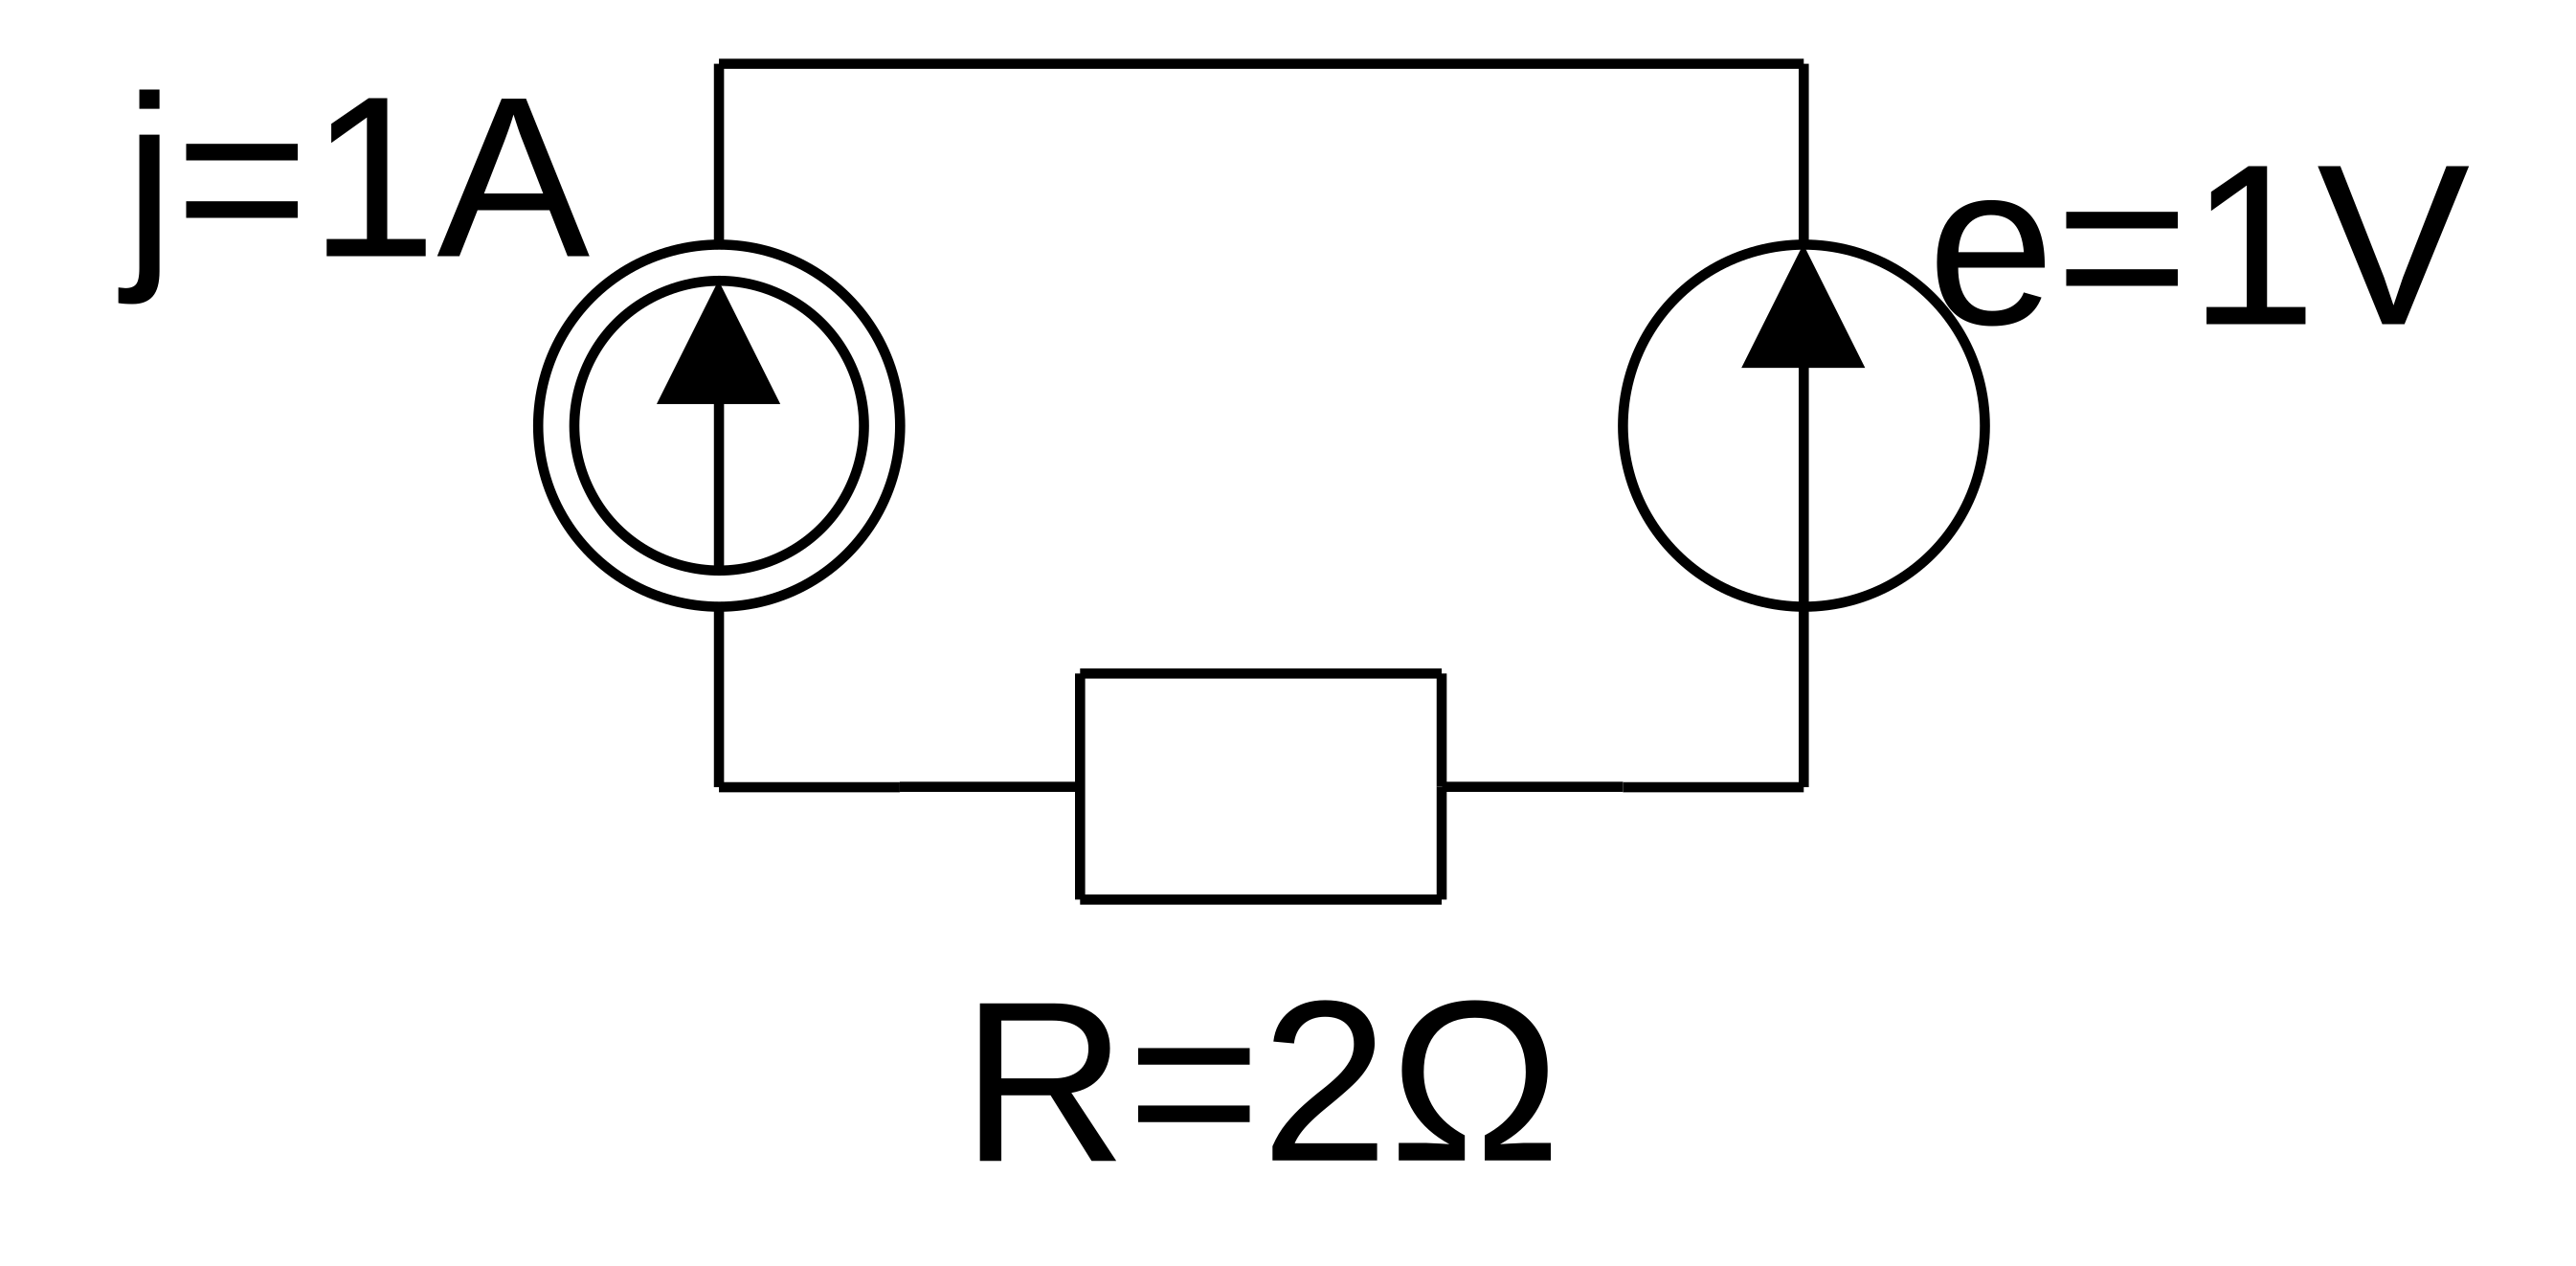
\includegraphics[scale=0.12, alt={}]{./imags/E01/12.png}
		\caption{Zadanie 12. Wykonaj bilans mocy.}
	\end{figure}	
\end{frame}